\documentclass[amssymb,secnumarabic,twocolumn,aps]{revtex4}

% allows special characters (including æøå)
\usepackage[utf8]{inputenc}
%\usepackage [norsk]{babel} %if you write norwegian
\usepackage[english]{babel}  %if you write english

\usepackage{physics,amssymb}  % mathematical symbols (physics imports amsmath)
\usepackage{graphicx}         % include graphics such as plots
\graphicspath{{../figures}}  % set the path for figures
\usepackage{xcolor}           % set colors
\usepackage{hyperref}         % automagic cross-referencing 
\usepackage{float}			  % force placement of tables and figures
% Required packages for the diagram
\usepackage{tikz}
\usepackage{amsmath}
\usepackage{bm}
\usetikzlibrary{positioning, arrows.meta, calc}
% Required packages for theorem 
\usepackage{amsthm}
\newtheorem*{theorem}{Theorem}

% Required packages for algorithms and code listings
\usepackage{algorithm}
\usepackage{algpseudocode}
\usepackage{listings}


\begin{document}
\title{Feed-Forward Neural Networks for Regression and Classification\\
    \normalsize FYS-STK3155 - Project 2}
\date{November 9, 2026}
\author{Hassen M. Morad}
\affiliation{Honours Student, University of Oslo}
\email{hmmorad@student.matnat.uio.no}

\newpage

\begin{abstract}
    Feed-forward neural networks can model complex relationships by combining multiple layers of connected neurons. Their performance depend on network architecture and chosen activation functions and optimization method, with the risk that increasing network complexity can lead to overfitting. We studied this using Runge's function $f(x) = \frac{1}{1+25x^2}$ for regression and the MNIST dataset \cite{lecun2010mnist} for handwritten digit classification. We implemented a neural network from scratch using NumPy \cite{numpy}, including the backpropagation, activation functions, and gradient-based optimization methods.

    For regression, we investigated network depth, width, activation functions, learning rate, and $\ell_1$ and $\ell_2$ regularization using cross-validation. The selected unregularized sigmoid network with one hidden layer of 50 neurons achieved test MSE $0.01187$ and $R^2=0.9043$, giving lower error than OLS, Ridge and Lasso from Project~1 \cite{project1}. For MNIST, the selected network with two sigmoid hidden layers of 200 neurons and weak $\ell_2$ regularization achieved test accuracy $97.88\%$ and macro-$F_1=0.9787$. Scikit-learn's MLP achieved $97.66\%$ and $0.9766$, while our logistic model achieved $92.45\%$ and $0.9235$. Our results show that additional layers do not automatically improve performance, and that architecture, optimization and regularization must be selected together using validation data.
\end{abstract}

\maketitle

\section{Introduction}

Neural networks are inspired by the human brain, which consists of an estimated 100 billion neurons, with each neuron connected to thousands of others. In a similar way, neural networks combine simple computational units (called neurons) into connected layers, that can learn complex patterns from data \cite{ibm_neural_networks}.

The aim is to use these learned patterns to make accurate predictions on new observations. A network that is too simple may not capture all the relationships in the data, while a network that is too complex can overfit the training set. How fast the network learns and how well it generalizes to new data also depend on the chosen optimization method, learning rate and activation functions.

We investigate this with two different problems: regression with \emph{Runge's function} and classification with the MNIST dataset \cite{lecun2010mnist}. First, we use Runge's function, $f(x) = \frac{1}{1+25x^2}$, on $[-1,1]$ with $n=100$ samples and Gaussian noise $\sigma=0.1$, to study how well neural networks approximate a nonlinear function. We examine how the number of hidden layers and neurons affects the predictions, and compare different activation functions, including sigmoid, ReLU, and Leaky ReLU. We also compare the results with OLS, Ridge, and Lasso regression from Project 1 \cite{project1}.

We further investigate how regularization affects the performance of the network. Similar to Ridge and Lasso regression, we introduce $\ell_2$ and $\ell_1$ penalties on the network weights. The $\ell_2$ penalty discourages large weights, while the $\ell_1$ penalty can drive individual weights to zero \cite{lecturebook}. We compare these approaches to examine whether regularization improves generalization and reduces overfitting.

In addition to regression, we apply neural networks to the MNIST dataset \cite{lecun2010mnist}, which contains $70,000$ handwritten digit images. The task is to classify each image as one of ten digits, from zero to nine. We use a softmax output layer to obtain class probabilities and categorical cross-entropy as the loss function. We evaluate the classification performance using accuracy, precision, recall, and F1-score, and compare our network with multiclass logistic regression.

Selecting suitable hyperparameters is important for obtaining models that generalize well to unseen data. We therefore use $k$-fold cross-validation, where the data is divided into $k$ folds, with each fold used once as a validation set while the model is fitted on the remaining folds \cite{hastie}. We use this to compare network architectures, activation functions, learning rates, and regularization strengths.

We also compare different optimization methods, including standard gradient descent, RMSProp, and Adam. These methods use gradients of the loss function to update the network weights, but differ in how they calculate and adjust the updates. We implement the network and optimization algorithms from scratch using NumPy \cite{numpy}, and compare our implementation of backpropagation with automatic differentiation from JAX \cite{jax}. Our network is compared with \texttt{MLPClassifier}, and similarly, our logistic regression with \texttt{LogisticRegression} from Scikit-learn \cite{scikit-learn}.

Section \ref{section:methods} presents the theory for neural network, activation functions, loss functions, regularization, and optimization methods. Section \ref{section:Implementation} describes our implementation and setup. Section \ref{section:results} presents the results and discussion, first for regression and then for MNIST classification. Finally, Section \ref{section:conclusion} summarizes our findings. The code is available at \url{https://github.com/hmmorad/FYS-STK3155-Projects}.


\section{Methods}\label{section:methods}

In Project 1, we studied regression using OLS, Ridge, and Lasso, and investigated different gradient-based optimization methods, with and without regularization (see Methods in project 1 \cite{project1} for introduction to these). We use these regression models as benchmarks in this project and reuse the optimization methods when training the neural networks. In the following section, we describe the structure of a feed-forward neural network, how its parameters are trained, and how it can be used for classification.

\subsection{The Universal Approximation Theorem}

The universal approximation theorem describes the ability of neural networks to approximate continuous functions. Cybenko's theorem gives the following result:
\begin{theorem}[from Cybenko \cite{cybenko1989} and Hjorth-Jensen \cite{lecturebook}]
    Let $\sigma$ be a continuous sigmoidal function satisfying
    \begin{equation*}
        \lim_{z\to-\infty}\sigma(z)=0,
        \qquad
        \lim_{z\to+\infty}\sigma(z)=1.
    \end{equation*}
    Let $F:[0,1]^d\rightarrow\mathbb{R}$ be a continuous function on the unit cube in $d$ dimensions. Then, for every $\epsilon>0$, there exists a feed-forward neural network $f(\boldsymbol{x};\boldsymbol{\Theta})$ with a single hidden layer such that
    \begin{equation*}
        \sup_{\boldsymbol{x}\in[0,1]^d}
        \left|F(\boldsymbol{x})-
        f(\boldsymbol{x};\boldsymbol{\Theta})\right|
        <\epsilon,
    \end{equation*}
    where $\boldsymbol{\Theta}$ contains the weights and biases of the network \cite{lecturebook}.
\end{theorem}

In other words, a network with only one hidden layer can approximate any continuous function on a compact domain to any accuracy, provided it has enough hidden nodes. Later results extended this theorem to a wider class of activation functions, including ReLU and Leaky ReLU \cite{lecturebook}.

However, the theorem is an existence result. It does not specify how many neurons are needed, or whether an optimization algorithm will find the weights that give the desired approximation. In other words, it does not guarantee that the network will generalize well to unseen data.

\subsection{Feed-forward neural networks}


% Feed-forward neural network diagram, generated using TikZ with DeepSeek
%%%%%%% LLM-generated
% Tool: ChatGPT (November 2026)
% Role: Generated a feed-forward neural network diagram using TikZ
% Modifications: Size and layout adjusted for better fit in the document
% Prompt: Asked it to generate a feed-forward neural network diagram using TikZ, and sent an example png (from lecture notes) for reference.
\begin{figure*}[t]
    \centering
    \resizebox{0.75\textwidth}{!}{% 
        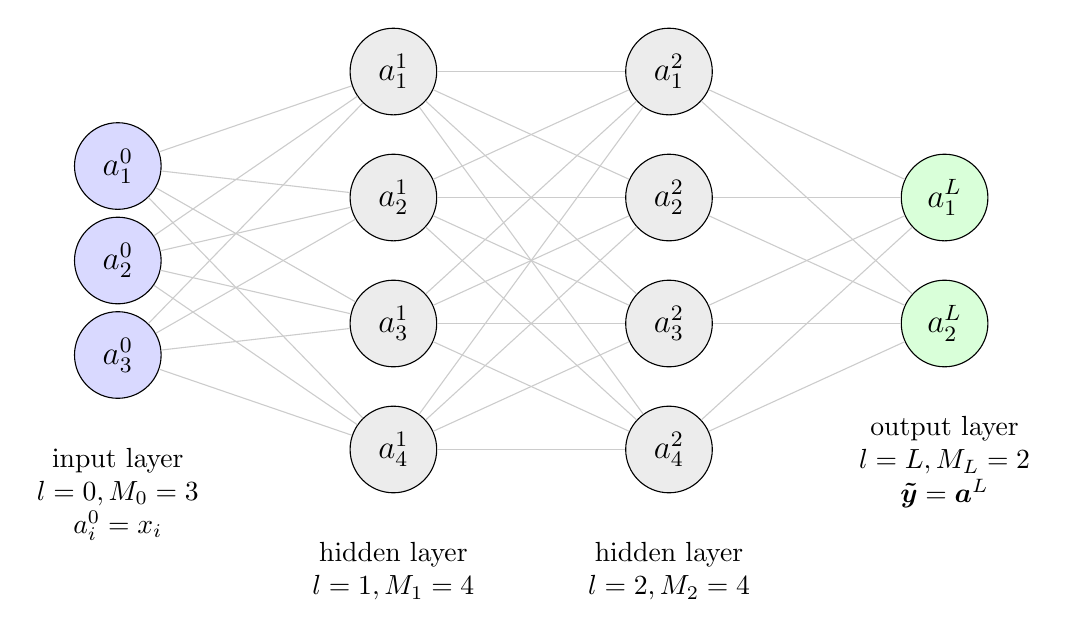
\begin{tikzpicture}[
            neuron/.style={circle, draw, minimum size=1.1cm, inner sep=0pt, font=\large},
            input neuron/.style={neuron, fill=blue!15},
            hidden neuron/.style={neuron, fill=gray!15},
            output neuron/.style={neuron, fill=green!15},
            connection/.style={draw=gray!40, thin},
            highlight/.style={draw=red, thick, -{Stealth[length=3mm]}}
            ]

            % --- 1. Define Nodes
            % Input Layer (l=0)
            \node[input neuron] (I1) at (0, 1.2) {\(a_1^0\)};
            \node[input neuron] (I2) at (0, 0) {\(a_2^0\)};
            \node[input neuron] (I3) at (0, -1.2) {\(a_3^0\)};
            % Hidden Layer 1 (l=1)
            \node[hidden neuron] (H11) at (3.5, 2.4) {\(a_1^1\)};
            \node[hidden neuron] (H12) at (3.5, 0.8) {\(a_2^1\)};
            \node[hidden neuron] (H13) at (3.5, -0.8) {\(a_3^1\)};
            \node[hidden neuron] (H14) at (3.5, -2.4) {\(a_4^1\)};
            % Hidden Layer 2 (l=2)
            \node[hidden neuron] (H21) at (7, 2.4) {\(a_1^2\)};
            \node[hidden neuron] (H22) at (7, 0.8) {\(a_2^2\)};
            \node[hidden neuron] (H23) at (7, -0.8) {\(a_3^2\)};
            \node[hidden neuron] (H24) at (7, -2.4) {\(a_4^2\)};
            % Output Layer (l=L)
            \node[output neuron] (O1) at (10.5, 0.8) {\(a_1^L\)};
            \node[output neuron] (O2) at (10.5, -0.8) {\(a_2^L\)};
            % --- 2. Draw Connections ---
            \foreach \i in {1,2,3} {
                    \foreach \j in {1,2,3,4} { \draw[connection] (I\i) -- (H1\j); }
                }
            \foreach \i in {1,2,3,4} {
                    \foreach \j in {1,2,3,4} { \draw[connection] (H1\i) -- (H2\j); }
                }
            \foreach \i in {1,2,3,4} {
                    \foreach \j in {1,2} { \draw[connection] (H2\i) -- (O\j); }
                }
            % --- 3. Labels ---
            \node[align=center, below=0.5cm of I3] {input layer\\ \(l=0, M_0 = 3\)\\ \(a_i^0 = x_i\)};
            \node[align=center, below=0.5cm of H14] {hidden layer\\ \(l=1, M_1 = 4\)};
            \node[align=center, below=0.5cm of H24] {hidden layer\\ \(l=2, M_2 = 4\)};
            \node[align=center, below=0.5cm of O2] {output layer\\ \(l=L, M_L = 2\)\\ \(\bm{\tilde{\bm{y}}} = \bm{a}^L\)};
        \end{tikzpicture}%
    }
    \caption{Architecture of a feed-forward neural network, with three neurons in the input layer, two hidden layers with four neurons each, and two neurons in the output layer. Made with TikZ, generated with DeepSeek.}
    \label{fig:neural_network}
\end{figure*}

A feed-forward neural network consists of an input layer, one or more hidden layers, and an output layer. Each layer contains nodes that receive values from the previous layer, calculate a weighted sum, add a bias, and then apply an activation function. In a fully connected network, every node is connected to all nodes in the preceding layer. Information is passed in one direction; from the input layer towards the output layer.

We number the layers from $l=0$ to $L$, where $l=0$ is the input layer and $l=L$ is the output layer. Let $M_l$ denote the number of nodes in layer $l$. The input to the network is represented by $\boldsymbol{a}^0=\boldsymbol{x}$. For node $j$ in layer $l$, the weighted sum and bias give the pre-activation
\begin{equation*}
    z_j^l =
    \sum_{i=1}^{M_{l-1}}w_{ij}^l a_i^{l-1}
    +b_j^l,
\end{equation*}
where $w_{ij}^l$ is the weight connecting node $i$ in layer $l-1$ to node $j$ in layer $l$, and $b_j^l$ is the corresponding bias. The activation of the node is then
\begin{equation*}
    a_j^l = f_l(z_j^l),
\end{equation*}
where $f_l$ is the activation function used in layer $l$. In matrix-vector form, these equations become:
\begin{align*}
    \boldsymbol{z}^l
     & = (\boldsymbol{W}^l)^T
    \boldsymbol{a}^{l-1}+\boldsymbol{b}^l, \\
    \boldsymbol{a}^l
     & = f_l(\boldsymbol{z}^l).
\end{align*}
The activation function is applied element-wise. Repeating these operations for $l=1,\ldots,L$ gives the network output $\boldsymbol{a}^L$, which represents the prediction.

In practice, the inputs are often arranged in a matrix $\boldsymbol{A}^{l-1}$, with one observation in each row. The feed-forward calculations for a batch of $n$ observations can then be written as
\begin{align*}
    \boldsymbol{Z}^l
     & = \boldsymbol{A}^{l-1}\boldsymbol{W}^l
    +\boldsymbol{b}^l,                        \\
    \boldsymbol{A}^l
     & = f_l(\boldsymbol{Z}^l).
\end{align*}
Here, the bias is added to each row of the matrix. This is the form used when processing multiple observations at once \cite{lecturebook}.

The non-linear activation functions are important for the network's ability to model complex relationships. If all layers instead use the identity function, $f_l(z)=z$, the network only consists of linear transformations and biases. For example, with two layers,
\begin{align*}
    \boldsymbol{a}^2
     & = (\boldsymbol{W}^2)^T
    \left((\boldsymbol{W}^1)^T\boldsymbol{x}
    +\boldsymbol{b}^1\right)+\boldsymbol{b}^2                                                \\
     & = \underbrace{(\boldsymbol{W}^1\boldsymbol{W}^2)^T}_{\boldsymbol{W}^T} \boldsymbol{x}
    + \underbrace{(\boldsymbol{W}^2)^T\boldsymbol{b}^1
        +\boldsymbol{b}^2}_{\boldsymbol{b}}.
\end{align*}
This is still an affine function of the input. The same applies when more linear layers are added, since their transformations can be combined into a single affine transformation. Thus, non-linear activation functions are necessary for the network to learn non-linear relationships \cite{lecturebook}.

\subsection{Activation functions}

We consider three activation functions in the hidden layers: sigmoid, ReLU, and Leaky ReLU. The sigmoid function (also often called the logistic function) maps its input to the interval $(0,1)$ and is defined as
\begin{equation*}
    \sigma(z)=\frac{1}{1+e^{-z}}.
\end{equation*}
Its derivative can be expressed in terms of the function itself:
\begin{equation*}
    \sigma'(z)=\sigma(z)(1-\sigma(z)).
\end{equation*}
The rectified linear unit (ReLU) is defined as
\begin{equation*}
    \text{ReLU}(z)=\max(0,z),
\end{equation*}
with derivative
\begin{equation*}
    \text{ReLU}'(z)=
    \begin{cases}
        1, & z>0, \\
        0, & z<0.
    \end{cases}
\end{equation*}
The derivative is undefined at $z=0$, where it is conventionally assigned to zero during implementation.

Leaky ReLU is a variation of ReLU that allows a small gradient when the input is negative. It is defined as
\begin{equation*}
    \text{LReLU}(z)=
    \begin{cases}
        z,        & z>0,     \\
        \alpha z, & z\leq 0,
    \end{cases}
\end{equation*}
where $\alpha$ is a small positive constant, commonly set to $0.01$. Its derivative is then
\begin{equation*}
    \text{LReLU}'(z)=
    \begin{cases}
        1,      & z>0,     \\
        \alpha, & z\leq 0.
    \end{cases}
\end{equation*}

The derivatives of these functions are used during backpropagation to calculate the gradients of the network parameters. The sigmoid derivative approaches zero for large positive and negative inputs. ReLU avoids this for positive inputs, but its derivative is zero for negative inputs. This can cause a neuron to stop updating if it only receives negative inputs. Leaky ReLU addresses this by retaining a small, non-zero derivative for negative inputs \cite{lecturebook}.

\subsection{Loss functions and backpropagation}

The network is trained by adjusting its weights and biases to minimize a cost function. The cost function measures the difference between the predicted values and the target values. Backpropagation is used to calculate the gradients of the cost function with respect to all weights and biases in the network. It applies the chain rule, starting at the output layer and moves backwards through the hidden layers.
\subsubsection{Loss functions}

We first consider one observation, and let $C$ denote the cost for this observation. The cost for a batch is calculated by averaging over the observations.

For regression, we use a linear output activation, also called the identity function,
\begin{equation*}
    f_L(z)=z,
    \qquad
    f_L'(z)=1.
\end{equation*}
Together with the mean squared error, the half-squared error for one observation is
\begin{equation*}
    C(a^L,y) = \frac{1}{2}(a^L-y)^2,
\end{equation*}
where $a^L$ is the prediction and $y$ is the target value.
The derivative with respect to the output activation is
\begin{equation*}
    \frac{\partial C}{\partial a^L} = a^L-y.
\end{equation*}
By the chain rule, the derivative with respect to the
pre-activation is
\begin{align*}
    \delta^L
     & = \frac{\partial C}{\partial z^L} \\
     & = \frac{\partial C}{\partial a^L}
    \frac{\partial a^L}{\partial z^L}    \\
     & = (a^L-y)\cdot 1                  \\
     & = a^L-y.
\end{align*}

A similar simplification occurs for classification when the output activation and loss function are chosen together. For binary classification, sigmoid activation is used with binary cross-entropy,
\begin{equation*}
    C(\boldsymbol{a}^L,\boldsymbol{y})=-y\log(a^L)-(1-y)\log(1-a^L),
\end{equation*}
where $a^L=\sigma(z^L)$. Applying the chain rule gives
\begin{align*}
    \frac{\partial C}{\partial z^L}
     & =
    \left(
    -\frac{y}{a^L}
    +\frac{1-y}{1-a^L}
    \right)a^L(1-a^L) \\
     & =a^L-y.
\end{align*}

For multiclass classification, we instead use $K$ output nodes, where $K$ is the number of classes. The softmax function converts the output scores into class probabilities:
\begin{equation*}
    a_k^L
    = \frac{\exp(z_k^L)}
    {\sum_{m=1}^{K}\exp(z_m^L)}.
\end{equation*}
The probabilities are non-negative and sum to one. For one observation with a one-hot encoded target $\boldsymbol{y}$, the categorical cross-entropy is
\begin{equation*}
    C(\boldsymbol{a}^L,\boldsymbol{y})
    = -\sum_{k=1}^{K}y_k\log(a_k^L).
\end{equation*}
This is one cost for the observation, calculated using all output nodes.

Each softmax output depends on all output pre-activations. The derivative is therefore
\begin{equation*}
    \frac{\partial a_k^L}{\partial z_j^L}
    = a_k^L\left(I(k=j)-a_j^L\right),
\end{equation*}
where $I(k=j)$ is one when $k=j$ and zero otherwise Applying the chain rule gives \cite{mehta2023softmax}:
\begin{align*}
    \delta_j^L
     & = \frac{\partial C}{\partial z_j^L} \\
     & = \sum_{k=1}^{K}
    \frac{\partial C}{\partial a_k^L}
    \frac{\partial a_k^L}{\partial z_j^L}  \\
     & = -\sum_{k=1}^{K}
    \frac{y_k}{a_k^L}
    a_k^L\left(I(k=j)-a_j^L\right)         \\
     & = -y_j+a_j^L\sum_{k=1}^{K}y_k       \\
     & = a_j^L-y_j,
\end{align*}
where we use $\sum_{k=1}^{K}y_k=1$.

Thus, for all three combinations considered, the output error is the difference between the prediction and the target:
\begin{equation}
    \boldsymbol{\delta}^L
    = \frac{\partial C}{\partial\boldsymbol{z}^L}
    = \boldsymbol{a}^L-\boldsymbol{y}.
\end{equation}

For a batch of $N$ observations, the mean cost is
\begin{equation*}
    C_{\mathrm{data}}
    = \frac{1}{N}\sum_{r=1}^{N}C_r,
\end{equation*}
where $C_r$ is the cost for observation $r$. The gradients are therefore averaged over the batch.

\subsubsection{Backpropagation}

% Backpropagation diagram generated using TikZ with DeepSeek
%%%%%%% LLM-generated
% Tool: ChatGPT (November 2026)
% Role: Generated backpropagation diagram using TikZ
% Modifications: Size and layout adjusted for better fit in the document. It also got the red arrows wrong, so fixed that.
% Prompt: Asked it to generate a backpropagation neural network diagram using TikZ, and sent an example png (from lecture notes) for reference.
\begin{figure*}[t]
    \centering
    \resizebox{\columnwidth}{!}{%
        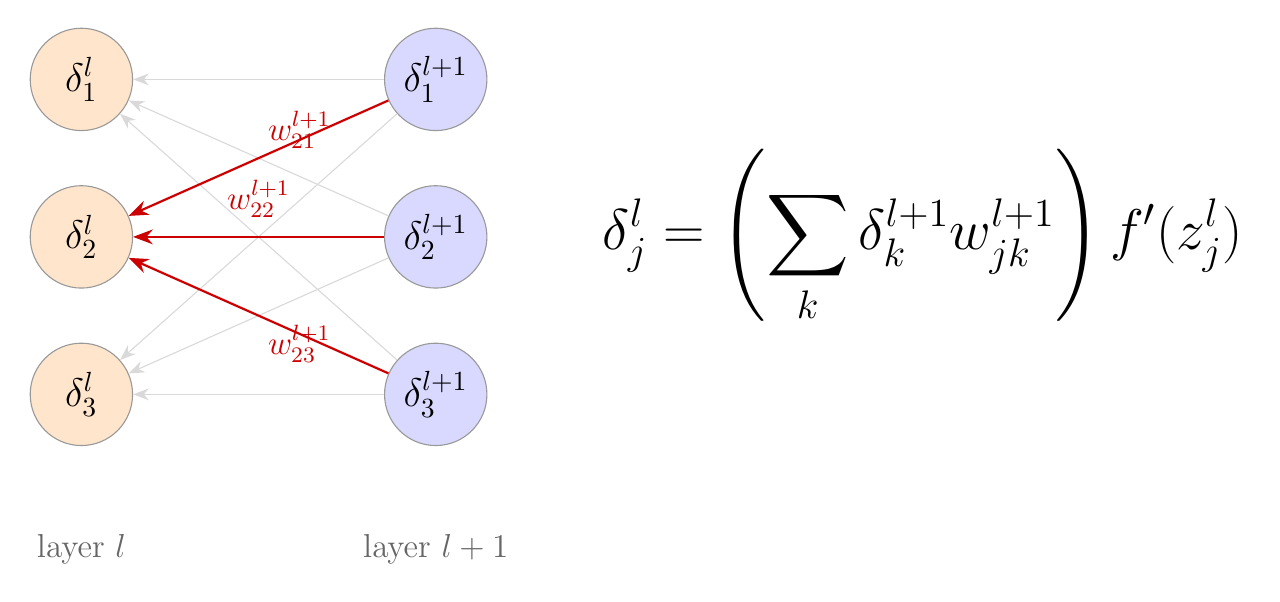
\begin{tikzpicture}[
            node base/.style={circle, draw=gray!80, minimum size=1.3cm, inner sep=0pt, font=\Large},
            left node/.style={node base, fill=orange!20},
            right node/.style={node base, fill=blue!15},
            gray conn/.style={draw=gray!30, thin, -{Stealth[length=2mm]}},
            red conn/.style={draw=red!80!black, thick, -{Stealth[length=2.5mm]}}
            ]

            % Nodes for Layer l
            \node[left node] (L1) at (0, 2) {\(\delta_1^l\)};
            \node[left node] (L2) at (0, 0) {\(\delta_2^l\)};
            \node[left node] (L3) at (0, -2) {\(\delta_3^l\)};

            % Nodes for Layer l+1
            \node[right node] (R1) at (4.5, 2) {\(\delta_1^{l+1}\)};
            \node[right node] (R2) at (4.5, 0) {\(\delta_2^{l+1}\)};
            \node[right node] (R3) at (4.5, -2) {\(\delta_3^{l+1}\)};

            % Background Gray Connections
            \foreach \i in {1,2,3} {
                    \foreach \j in {1,2,3} {
                            \draw[gray conn] (R\i) -- (L\j);
                        }
                }

            % Highlighted Red Connections
            \draw[red conn] (R1) -- node[above right=0.1cm, inner sep=1pt, text=red!80!black, font=\large] {\(w_{21}^{l+1}\)} (L2);
            \draw[red conn] (R2) -- node[above=0.2cm, inner sep=1pt, text=red!80!black, font=\large] {\(w_{22}^{l+1}\)} (L2);
            \draw[red conn] (R3) -- node[below right=0.1cm, inner sep=1pt, text=red!80!black, font=\large] {\(w_{23}^{l+1}\)} (L2);

            % Layer Labels
            \node[below=1cm of L3, text=gray!80!black, font=\large] {layer \(l\)};
            \node[below=1cm of R3, text=gray!80!black, font=\large] {layer \(l+1\)};

            % Equation on the right
            \node[anchor=west, font=\huge] at (6.5, 0) {
                \(\displaystyle \delta_j^l = \left( \sum_k \delta_k^{l+1} w_{jk}^{l+1} \right) f'(z_j^l)\)
            };

        \end{tikzpicture}%
    }
    \caption{Backward pass of the error signal through the network. Made with TikZ, generated with DeepSeek.}
    \label{fig:backward_pass}
\end{figure*}

The forward pass has already calculated the pre-activations $\boldsymbol{z}^l$ and activations $\boldsymbol{a}^l$ for every layer. These values are stored and reused during backpropagation. The pre-activations are needed to evaluate the derivatives of the activation functions, while the activations from the previous layer are needed to calculate the weight gradients.

We can see this by considering the error in a hidden layer. The pre-activation of node $j$ in layer $l$ affects the cost through its activation $a_j^l$. This activation is connected to every node $k$ in the next layer.  We define the error of node $j$ in layer $l$ as
\begin{equation*}
    \delta_j^l
    =\frac{\partial C}{\partial z_j^l}.
\end{equation*}
Applying the chain rule gives
\begin{align*}
    \delta_j^l
     & =\frac{\partial C}{\partial z_j^l} \\
     & =\sum_{k=1}^{M_{l+1}}
    \frac{\partial C}{\partial z_k^{l+1}}
    \frac{\partial z_k^{l+1}}{\partial a_j^l}
    \frac{\partial a_j^l}{\partial z_j^l} \\
     & =f_l'(z_j^l)
    \sum_{k=1}^{M_{l+1}}
    w_{jk}^{l+1}\delta_k^{l+1}.
\end{align*}
The error in layer $l$ is therefore calculated using the errors in the layer after (i.e., $l+1$), and the corresponding weights and derivative of the activation function. In matrix-vector form:
\begin{equation*}
    \boldsymbol{\delta}^l
    =
    \left(\boldsymbol{W}^{l+1}
    \boldsymbol{\delta}^{l+1}\right)
    \circ f_l'(\boldsymbol{z}^l),
\end{equation*}

where $\circ$ denotes element-wise multiplication.

Once the errors have been calculated, the gradients with respect to the weights and biases follow from the derivatives of the pre-activation:
\begin{equation*}
    \frac{\partial z_j^l}{\partial w_{ij}^l}
    =a_i^{l-1},
    \qquad
    \frac{\partial z_j^l}{\partial b_j^l}=1.
\end{equation*}
Using the chain rule, we therefore obtain
\begin{align*}
    \frac{\partial C}{\partial w_{ij}^l}
     & =\frac{\partial C}{\partial z_j^l}
    \frac{\partial z_j^l}{\partial w_{ij}^l}
    =\delta_j^l a_i^{l-1},                \\
    \frac{\partial C}{\partial b_j^l}
     & =\frac{\partial C}{\partial z_j^l}
    \frac{\partial z_j^l}{\partial b_j^l}
    =\delta_j^l.
\end{align*}

Once the gradients have been calculated using backpropagation, the weights and biases are updated to reduce the cost function. With standard gradient descent and learning rate $\gamma$, the updates are
\begin{align*}
    w_{ij}^l
     & \leftarrow
    w_{ij}^l-\gamma
    \frac{\partial C}{\partial w_{ij}^l}, \\
    b_j^l
     & \leftarrow
    b_j^l-\gamma
    \frac{\partial C}{\partial b_j^l}.
\end{align*}
Without regularization, the weight update becomes:
\begin{equation*}
    w_{ij}^l
    \leftarrow
    w_{ij}^l-\gamma\delta_j^l a_i^{l-1}.
\end{equation*}

The optimization methods for neural networks are based on the same algorithms studied in Project 1 \cite{project1}.

\subsection{Regularization and weight initialization}

As the number of layers and nodes increases, a neural network can become more complex and may overfit the training data. Similar to Ridge and Lasso regression in Project 1, we can introduce regularization terms to penalize large weights. The two cost functions are then:
\begin{align*}
    C_{\ell_1}
     & =C_{\mathrm{data}}
    +\lambda\sum_{l=1}^{L}\|\boldsymbol{W}^l\|_1, \\
    C_{\ell_2}
     & =C_{\mathrm{data}}
    +\lambda\sum_{l=1}^{L}\|\boldsymbol{W}^l\|_2^2,
\end{align*}
where $C_{\mathrm{data}}$ is the original cost function and $\lambda$ controls the strength of regularization. The $\ell_1$ penalty can encourage individual weights to become zero, while the $\ell_2$ penalty shrinks weights towards zero.

The regularization gets added to the gradients obtained from backpropagation. For $\ell_1$ regularization, the gradient with respect to a weight becomes
\begin{equation*}
    \frac{\partial C_{\ell_1}}{\partial w_{ij}^l}
    =
    \delta_j^l a_i^{l-1}
    +\lambda\operatorname{sign}(w_{ij}^l),
\end{equation*}
For $\ell_2$ regularization, the corresponding gradient is
\begin{equation*}
    \frac{\partial C_{\ell_2}}{\partial w_{ij}^l}
    =
    \delta_j^l a_i^{l-1}+2\lambda w_{ij}^l.
\end{equation*}
The regularization terms do not depend on the biases, so their gradients remain unchanged. The penalties therefore only add an extra term to the weight gradients, while the backpropagation calculation of the errors remains the same \cite{lecturebook}.

The initial weights also affect how well a network can be trained. If all weights are initialized to zero, the nodes in the same layer receive identical gradients and remain identical during training. The weights must therefore be initialized with different values. At the same time, weights that are too large can make the activations saturate, while weights that are too small can cause the signal and gradients to become very small \cite{lecturebook}.

Xavier initialization of the weights, by Glorot and Bengio \cite{Xavier2010}, aims to preserve the variance of the activations during the forward pass and the gradients during the backward pass. It uses weights, drawn from a Gaussian or uniform distribution \cite{lecturebook}, with mean zero and variance
\begin{equation*}
    \operatorname{Var}(w_{ij}^l)
    =\frac{2}{M_{l-1}+M_l}.
\end{equation*}
For ReLU and Leaky ReLU, He initialization \cite{He2015} accounts for the fact that ReLU sets approximately half of its inputs to zero. It therefore uses the variance
\begin{equation*}
    \operatorname{Var}(w_{ij}^l)
    =\frac{2}{M_{l-1}}.
\end{equation*}

These initialization methods help maintain the scale of activations and gradients across layers. Biases are commonly initialized to zero, or to a small positive value when using ReLU \cite{lecturebook}.

\subsection{Vanishing and exploding gradients}

The backpropagation equations involve repeated multiplication by weight matrices and derivatives of activation functions. This can cause the gradients to become either very small or very large as they are propagated backwards through the network.

To see this, define $\boldsymbol{D}^l$ as a diagonal matrix containing the derivatives of the activation function in layer $l$. The hidden-layer error can then be written as
\begin{equation*}
    \boldsymbol{\delta}^l
    =\boldsymbol{D}^l
    \boldsymbol{W}^{l+1}
    \boldsymbol{\delta}^{l+1}.
\end{equation*}
Applying this recursively gives
\begin{equation*}
    \boldsymbol{\delta}^l
    =
    \boldsymbol{D}^l\boldsymbol{W}^{l+1}
    \boldsymbol{D}^{l+1}\boldsymbol{W}^{l+2}
    \cdots
    \boldsymbol{D}^{L-1}\boldsymbol{W}^{L}
    \boldsymbol{\delta}^{L}.
\end{equation*}

The gradient reaching an early layer is therefore a product of many weight matrices and activation derivatives. If these factors repeatedly reduce the magnitude of the gradient, it becomes very small. This is known as the vanishing gradient problem. The weights in the early layers then receive very small updates and learn slowly. If the factors instead increase the magnitude, the gradients can become very large, causing excessively large parameter updates and unstable training. This is known as the exploding gradient problem \cite{lecturebook}.

The sigmoid function can contribute to vanishing gradients because its derivative is at most $1/4$ and approaches zero for large positive and negative inputs. Repeated multiplication by these derivatives can therefore strongly reduce the gradients in deeper layers. ReLU avoids this for positive inputs, since its derivative is one, but can produce zero gradients for negative inputs. Leaky ReLU retains a small derivative for negative inputs, reducing the risk of neurons becoming inactive \cite{lecturebook}.

\subsection{Logistic regression and classification metrics}

Logistic regression is used as a baseline for the MNIST classification task. In the multiclass setting, the model calculates a score for each class using a linear combination of the input features:
\begin{equation*}
    \boldsymbol{z}
    =\boldsymbol{W}^T\boldsymbol{x}+\boldsymbol{b}.
\end{equation*}
The scores are converted into class probabilities using the softmax function.

Logistic regression can be viewed as a feed-forward neural network with no hidden layers, where the input layer is connected directly to the softmax output layer. In a neural network, the final softmax layer performs logistic regression on the learned features in the hidden layers rather than on the original input. Logistic regression is then a useful baseline for evaluating whether the additional complexity of a neural network and its hidden layers improves performance \cite{lecturebook}.

\subsubsection{Classification metrics}

We evaluate classification performance using accuracy, the confusion matrix, precision, recall, and the $F_1$-score. The confusion matrix compares the true class labels with the predicted labels. For a problem with $K$ classes, the entry in row $i$ and column $j$ counts the observations belonging to class $i$ that were predicted as class $j$. The diagonal therefore contains the correctly classified observations, while the off-diagonal entries show the classification errors.

Accuracy measures the proportion of correctly classified observations:
\begin{equation*}
    \mathrm{Accuracy}
    =\frac{1}{n}\sum_{i=1}^{n}
    I(\tilde{y}_i=y_i),
\end{equation*}
where $I(\cdot)$ is the indicator function, $\tilde{y}_i$ is the predicted class, and $y_i$ is the true class.

Precision and recall measure different types of classification errors. Precision is the proportion of predicted positives that are correct, while recall is the proportion of actual positives that are correctly identified:
\begin{align*}
    \mathrm{Precision}
     & =\frac{\mathrm{TP}}{\mathrm{TP}+\mathrm{FP}}, \\
    \mathrm{Recall}
     & =\frac{\mathrm{TP}}{\mathrm{TP}+\mathrm{FN}},
\end{align*}
where $\mathrm{TP}$, $\mathrm{FP}$, and $\mathrm{FN}$ denote true positives, false positives, and false negatives, respectively. The $F_1$-score is the harmonic mean of precision and recall:
\begin{equation*}
    F_1=
    2\frac{\mathrm{Precision}\cdot\mathrm{Recall}}
    {\mathrm{Precision}+\mathrm{Recall}}.
\end{equation*}

For multiclass classification, these measures are calculated separately for each class by treating that class as the positive class and all other classes as negative. We report macro-averaged precision, recall, and $F_1$-score, which are calculated as the arithmetic mean of the corresponding scores across all classes. The confusion matrix is particularly useful for interpreting these results, since it shows which digit classes are most often confused \cite{lecturebook}.


\section{Implementation}\label{section:Implementation}

Our implementation of the feed-forward neural network is organized into separate classes for the network layers, activation functions, loss functions, optimizers, and training procedure. This makes it possible to change the network architecture, activation functions, and optimization method without changing the overall training procedure.

\subsection{Neural network and training}

The network is implemented using two main classes: \texttt{DenseLayer} and \texttt{NeuralNetwork}. The \texttt{DenseLayer} class represents a fully connected layer and stores its weight matrix, bias vector, and activation function.
The weights are initialized using Xavier or He initialization (sampled from a normal distribution), depending on the activation function, as discussed in Section~\ref{section:methods}. In our implementation, the biases are initialized to $0.01$. A random seed is used to make the initialization reproducible.

The \texttt{NeuralNetwork} class combines the layers and handles the forward and backward passes. It also calculates the loss and includes the $\ell_1$ and $\ell_2$ regularization terms in the cost function and weight gradients.

The network's \texttt{forward()} method passes the input through all layers, while \texttt{backward()} iterates through the layers in reverse order and calculates the gradients. The loss gradient for the output layer is initialized as
\begin{equation*}
    \frac{\partial C}{\partial\boldsymbol{a}^L}
    =
    \boldsymbol{a}^L-\boldsymbol{y},
\end{equation*}

since we use the natural activation and loss combinations, as described in Section~\ref{section:methods}. We divide by $N$ to obtain the average gradient over the batch, where $N$ is the batch size.

Training is handled separately by the \texttt{NetworkTrainer} class. It receives the network configuration, optimizer, learning rate and other training parameters. This separates the training process from the network architecture and makes it possible to use different optimizers with the same network.

An example of how the trainer is initialized is shown below:

\begin{lstlisting}[language=Python, title={Example of initializing a neural network with NetworkTrainer. Layer architecture based on figure \ref{fig:neural_network}.}]
network_kwargs = {
    "n_inputs": 3,
    "layers": (
        (4, ReLU),
        (4, ReLU),
        (2, Softmax), # Output layer
    ),
    "lmbd1": 0.0,
    "lmbd2": 0.0,
    "seed": 2026,
}

trainer = NetworkTrainer(
    network_kwargs=network_kwargs,
    optimizer=Adam,
    optimizer_kwargs={"gamma": 0.01},
    epochs=100,
    batch_size=64,
    seed=2026,
)
\end{lstlisting}

To train, we call the \texttt{fit()} method, and pass in the training data, and optionally a validation dataset. This method handles the forward and backward passes and parameter updates. It returns a history \texttt{dict} containing the training (and optionally validation) loss for each epoch.

\subsection{Data preparation and cross-validation}

For the regression problem, we use the same Runge data and training and test split as in Project 1 ($80/20$ split). The data is scaled before training, following the same approach as in Project 1 \cite{project1}. When performing cross-validation, the scaling parameters are estimated using only the training fold and then applied to the validation fold to avoid data leakage.

For MNIST, each image is flattened from a $28\times 28$ matrix into a vector of $784$ input features. The pixel values, originally between $0$ and $255$, are scaled to the interval $[0,1]$. We use the original split of $60\,000$ training images and $10\,000$ test images. Like with regression, hyperparameter selection is performed using only the training data, and leaving the test set untouched until the final evaluation.

We use Scikit-learn's \texttt{KFold()} implementation for our cross-validation \cite{scikit-learn}. A new network and trainer are initialized for each fold, ensuring that each model starts with independently initialized parameters. The mean validation score and standard error across the folds are used to compare different hyperparameter configurations. Our \texttt{CrossValidation} class handles this procedure and allows us to evaluate different architectures, activation functions, learning rates, and regularization strengths.

The data is split into training and test sets using Scikit-learn's \texttt{train\_test\_split()} function, while cross-validation is performed using \texttt{KFold()} \cite{scikit-learn}. The test set is kept separate from model selection and is only used for the final evaluation. We also used \texttt{confusion\_matrix} and \texttt{f1\_score} from Scikit-learn to evaluate the classification performance on the MNIST dataset.

\subsection{Testing and verification}

An important part of implementing a neural network is checking that the calculated gradients and predictions are correct. We therefore perform several tests to verify our implementation.

First, we compare the analytical gradients from backpropagation with gradients calculated using automatic differentiation with JAX \cite{jax}. This allows us to check the gradients for individual weights and biases on a small network. We also test our CrossValidation implementation to ensure that it correctly splits the data and aggregates the validation scores across folds.

We also compare our implementation with Scikit-learn's \texttt{MLPClassifier} and \texttt{LogisticRegression} for MNIST classification \cite{scikit-learn}. These tests are compared against our results in the result section.

The tests are located in the \texttt{tests/} directory of the \texttt{project2/} package and are run through \texttt{Project2\_tests.ipynb}, located in the \texttt{Notebooks/} directory. The experiments and figures presented in the Results section are generated using \texttt{Project2\_results.ipynb}, which also saves the resulting figures.

\section{Results and Discussion}\label{section:results}

We first check the backpropagation gradients against automatic differentiation with JAX, as described in Section~\ref{section:Implementation}. We also test our CrossValidation implementation. The tests are run in \texttt{Project2\_tests.ipynb}, and pass successfully.

\subsection{Regression}\label{sec:results_regression}

For regression, we use the same 80 training points and 20 test points as in Project~1, with noise standard deviation $\sigma=0.1$ and seed $2026$. For the OLS, Ridge and Lasso baselines, we reuse the polynomial degrees and regularization strengths selected in Project~1, together with their CV MSE and SE. These models are refitted on the 80 training points for the final comparison.

All reported MSE values exclude the regularization penalty. The cross-validation (CV) results are the mean validation MSE over five folds, together with the standard error (SE). The test set is not used for hyperparameter selection and is only evaluated after the model choices are fixed.

\subsubsection{Comparison with polynomial regression}

We first compare our network with one sigmoid hidden layer of 50 neurons against degree-10 OLS and Scikit-learn's MLP (Figure~\ref{fig:regression_50}). Scikit-learn's MLP was initialized with the same architecture as our network. Our network gives training $R^2=0.856$, compared with $0.854$ for Scikit-learn and $0.851$ for OLS. Our network therefore slightly outperforms the alternatives on the training set. The difference between our network and Sklearn's MLP can be attributed to the random initialization of the weights. All three training MSE values are approximately $0.014$-$0.015$, but we see OLS oscillates near the boundaries. The network has learned the underlying function more smoothly than OLS near the boundaries.

Increasing to two hidden layers of 100 neurons gives little visible improvement (Figure~\ref{fig:regression_100}). Both larger networks give training MSE approximately $0.0141$ and $R^2=0.857$, but the parameter count increases from 151 to 10\,401. For these 80 training points, the larger network therefore gives little improvement at the tested settings.

\begin{figure}[!htbp]
    \centering
    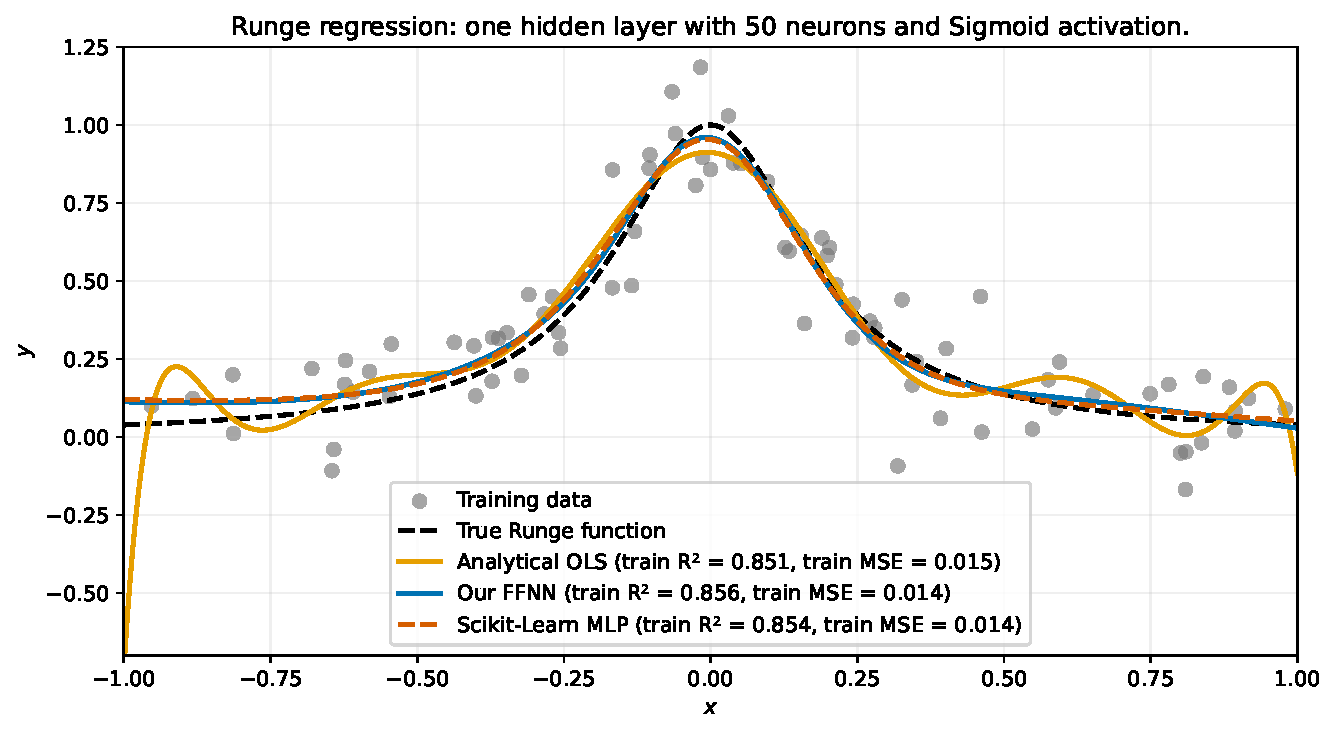
\includegraphics[width=\columnwidth]{part_b_comparison_50.pdf}
    \caption{Our FFNN and Scikit-learn's MLP give nearly overlapping Runge fits, while degree-10 OLS oscillates near the boundaries. Both networks use one sigmoid hidden layer with 50 neurons, a linear output, Adam with $\gamma=0.01$, full batches of 80 points and 1000 epochs. The legend shows training $R^2$ and MSE.}
    \label{fig:regression_50}
\end{figure}

\begin{figure}[!htbp]
    \centering
    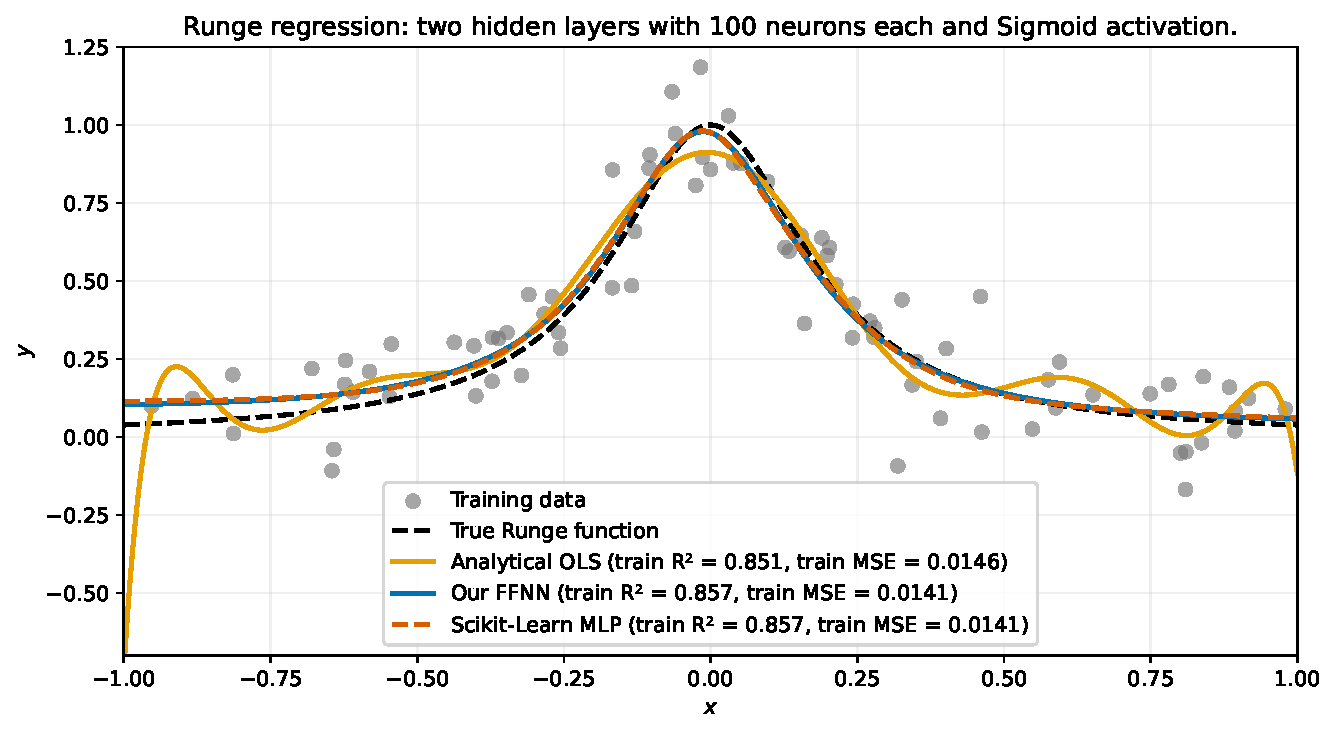
\includegraphics[width=\columnwidth]{part_b_comparison_100.pdf}
    \caption{Our FFNN and Scikit-learn's MLP give nearly overlapping Runge fits, while degree-10 OLS oscillates near the boundaries. Both networks use two sigmoid hidden layers with 100 neurons each, a linear output, Adam with $\gamma=0.01$, full batches of 80 points and 1000 epochs. The legend shows training $R^2$ and MSE.}
    \label{fig:regression_100}
\end{figure}

\subsubsection{Learning rate and optimization}

\begin{figure}[!htbp]
    \centering
    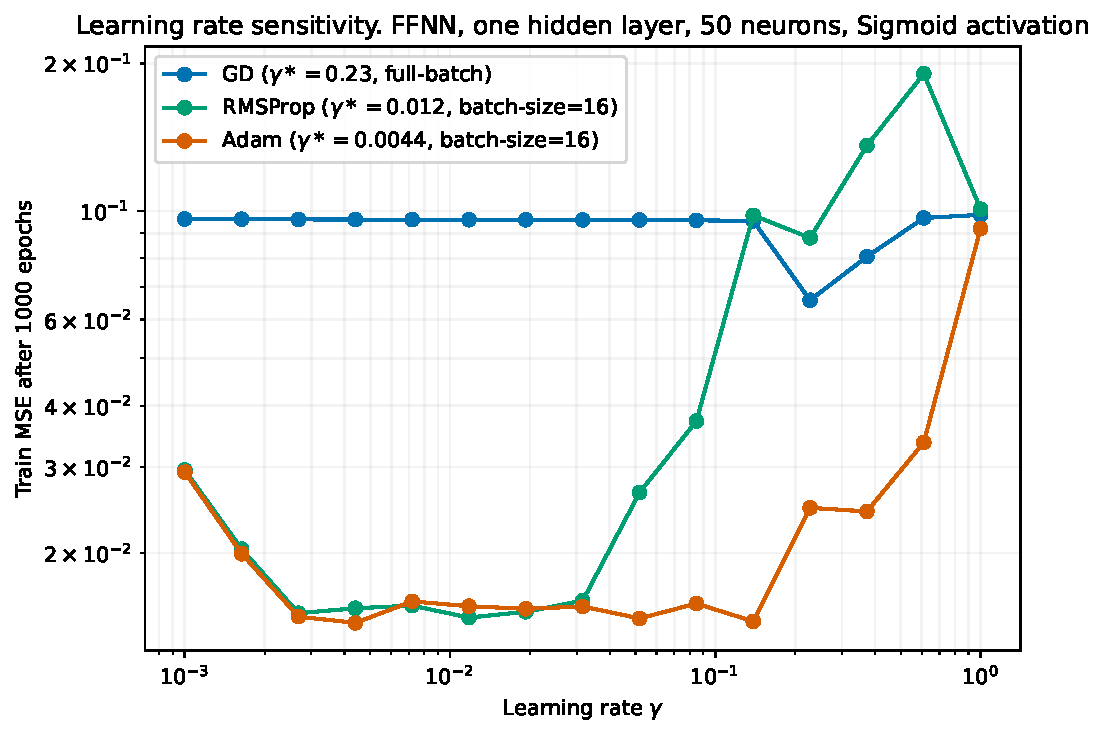
\includegraphics[width=\columnwidth]{part_b_training_mse_gamma_50.pdf}
    \caption{Adam reaches low training MSE over a broader range of learning rates than RMSProp. Each network has one sigmoid hidden layer of 50 neurons and is trained for 1000 epochs. GD uses full batches of 80 points, while Adam and RMSProp use batches of 16.}
    \label{fig:regression_learning_rate}
\end{figure}

Figure~\ref{fig:regression_learning_rate} show how the learning rate affects training. Adam reaches a training MSE near $0.015-0.020$ over a relatively broad range of rates. RMSProp reaches similar errors, but its error increases earlier as the rate becomes larger. Plain GD stays close to $0.10$ over much of the grid. Its best tested rate, $\gamma\approx0.23$, reduces the MSE to approximately $0.060$ after 1000 epochs, which is still above Adam and RMSProp, and converges slowly.

\begin{figure}[!htbp]
    \centering
    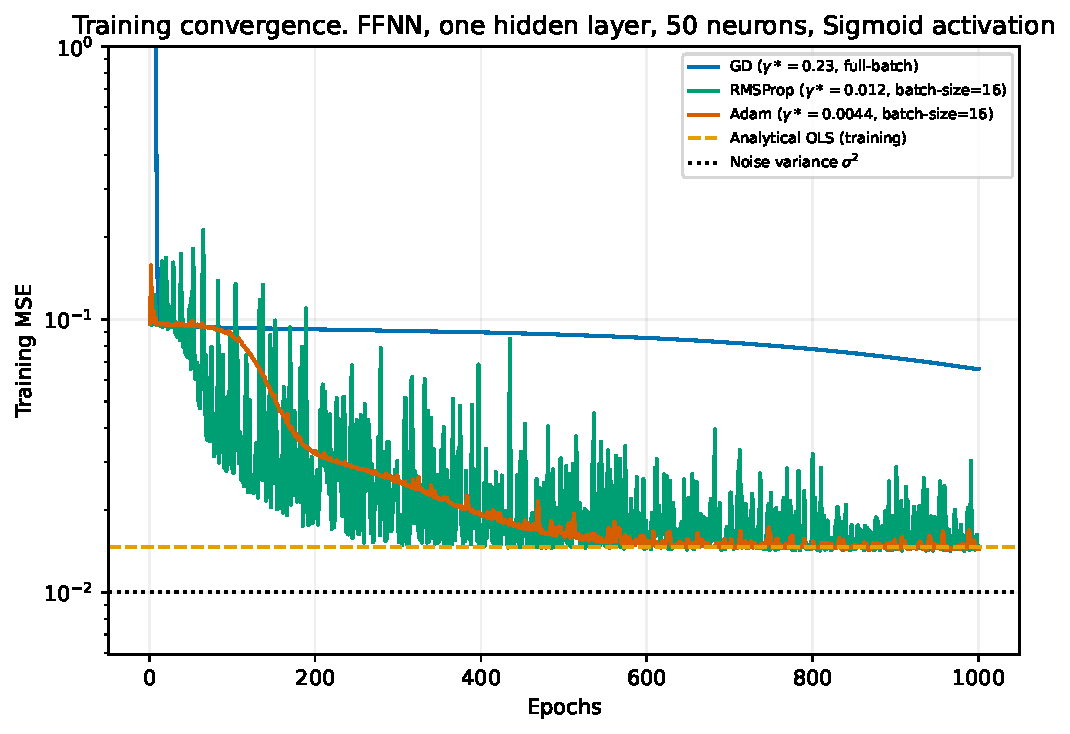
\includegraphics[width=\columnwidth]{part_b_optimizer_convergence_50.pdf}
    \caption{Adam learns more smoothly after its initial plateau, while RMSProp learns quickly but fluctuates throughout training. Each optimizer uses the learning rate giving its lowest training MSE after 1000 epochs: GD $\gamma\approx0.23$, RMSProp $\gamma\approx0.012$ and Adam $\gamma\approx0.0044$. The network has one sigmoid hidden layer of 50 neurons. GD uses full batches, while Adam and RMSProp use batches of 16. The horizontal lines show the OLS training MSE and noise variance $\sigma^2=0.01$.}
    \label{fig:regression_convergence}
\end{figure}

For each optimizer, we plot the training history at the rate with the lowest MSE after 1000 epochs (Figure~\ref{fig:regression_convergence}). RMSProp initially learns quickly, but its error fluctuates throughout training. Adam learns more smoothly after an initial plateau and approaches the OLS training error more stable over time compared with RMSProp. We therefore use Adam in the following experiments. GD makes one full-batch update per epoch, while Adam and RMSProp make five minibatch updates, so the effective number of weight updates per epoch differs between the optimizers.

\subsubsection{Activation, depth and width}

\begin{figure*}[!t]
    \centering
    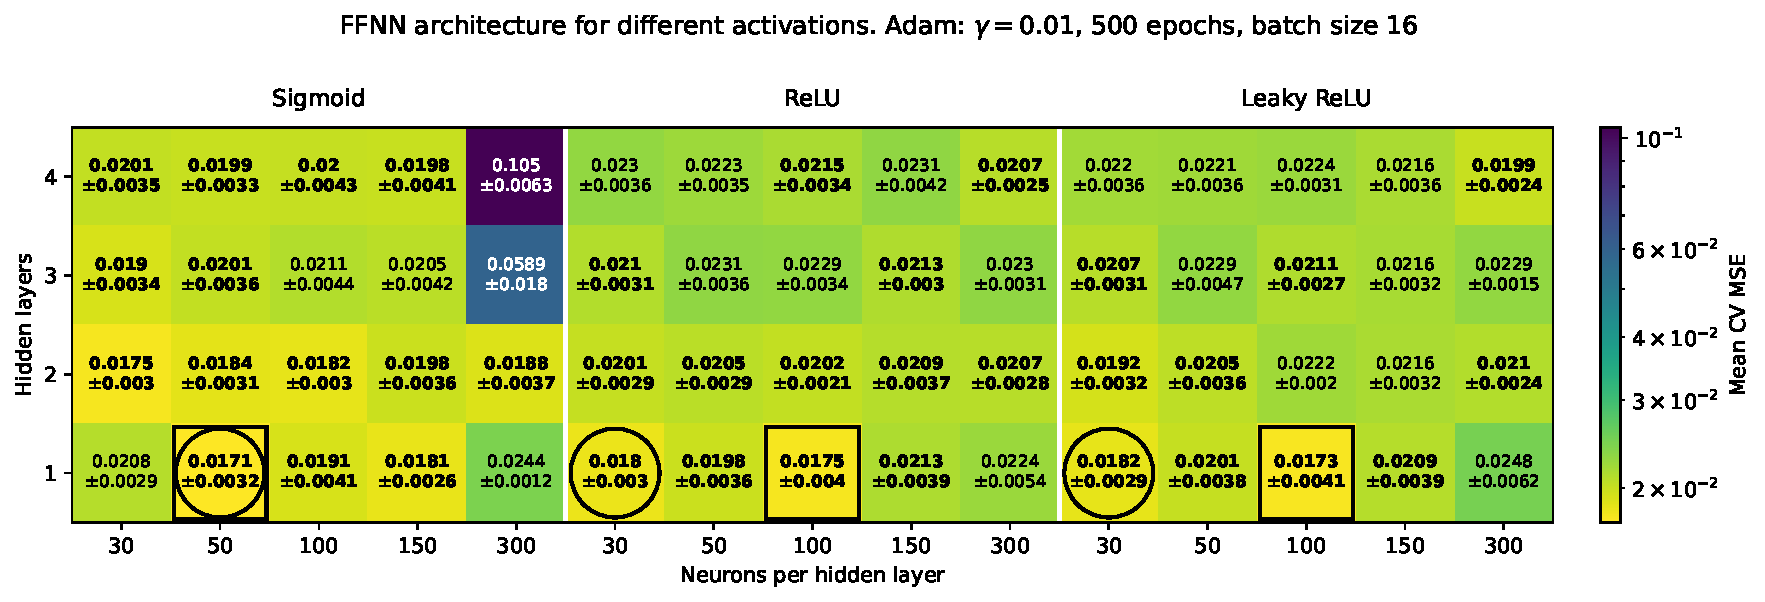
\includegraphics[width=\textwidth]{part_c_activations_cv.pdf}
    \caption{Adding layers usually gives higher CV MSE for the widest sigmoid networks. With 300 neurons per layer, the four-layer sigmoid network reaches approximately $0.105 \pm 0.0063$, compared with about $0.02\pm 0.0025$ for ReLU and Leaky ReLU. All models use Adam, $\gamma=0.01$, 500 epochs, batch size 16 and five-fold CV. Cells show mean validation MSE $\pm$ SE with the same logarithmic colour scale. For each activation, the square marks the minimum, the circle the one-SE choice, and bold cells are within one SE of the minimum.}
    \label{fig:regression_architecture}
\end{figure*}

In Figure~\ref{fig:regression_architecture}, we vary the activation function, number of hidden layers and neurons per layer. Increasing depth or width does not consistently reduce CV MSE. Sigmoid gives its lowest error with one hidden layer of 50 neurons, at approximately $0.0171\pm0.0032$. The lowest errors for ReLU and Leaky ReLU are $0.0175\pm0.0044$ and $0.0173\pm0.0041$. The differences are small compared with the SE. Using the one-SE rule separately for each activation selects one layer with 50 neurons for sigmoid and 30 neurons for ReLU and Leaky ReLU.

The effect of adding layers is clearest for sigmoid with 300 neurons per layer. CV MSE increases from approximately $0.0188$ with two layers to $0.0589$ with three and $0.105$ with four. ReLU and Leaky ReLU remain near $0.0207$ and $0.0199$ with four layers. This may be explained by vanishing gradients, as discussed in Section~\ref{section:methods}. The sigmoid derivative is at most $1/4$, and multiplying these derivatives through several layers can make the gradients small. Running the network for more epochs may help, but we have not tested this extensively.

We use 500 epochs for every configuration. With more epochs, some deeper sigmoid networks may learn more, but we have not tested whether they reach the same error as ReLU. A high CV MSE alone does not tell us whether the problem is slow learning or overfitting.


\subsubsection{Regularization}

We next test $\ell_1$ and $\ell_2$ regularization, using fewer architectures and varying the learning rate and penalty strength. The full heatmaps are in Appendix~\ref{app:regression_extra}. With strong regularization, $\lambda=0.1$, CV MSE is generally close to $0.10$. This suggests underfitting, since the penalty limits how much the model can vary. Weaker penalties give lower errors at suitable learning rates. Larger networks do not consistently improve the result and can be sensitive to the learning rate and number of epochs needed.

\begin{table*}[t]
    \centering
    \caption{One-standard-error selections for each activation and penalty. Bold rows have the lowest CV MSE among the three activation-specific selections for each penalty. Scores are mean validation MSE and SE.}
    \label{tab:part_d_selected_models}
    \begin{tabular}{llllllll}
        \hline\hline
        Penalty     & Activation       & Architecture   & Parameters   & $\gamma$      & $\lambda$       & CV MSE           & CV SE             \\
        \hline
        \textbf{L1} & \textbf{Sigmoid} & \textbf{(50,)} & \textbf{151} & \textbf{0.05} & \textbf{0.0001} & \textbf{0.01729} & \textbf{0.003953} \\
        L1          & ReLU             & (50,)          & 151          & 0.05          & 0.0001          & 0.01937          & 0.003305          \\
        L1          & Leaky ReLU       & (50,)          & 151          & 0.1           & 0.0001          & 0.01866          & 0.003992          \\
        L2          & Sigmoid          & (50,)          & 151          & 0.05          & 0.0001          & 0.01948          & 0.004988          \\
        \textbf{L2} & \textbf{ReLU}    & \textbf{(50,)} & \textbf{151} & \textbf{0.01} & \textbf{0.0001} & \textbf{0.01825} & \textbf{0.002843} \\
        L2          & Leaky ReLU       & (50,)          & 151          & 0.003         & 0.001           & 0.02063          & 0.003652          \\
        \hline\hline
    \end{tabular}
\end{table*}


Table~\ref{tab:part_d_selected_models} shows the one-SE choices for each activation and penalty. Among eligible models, we prefer fewer parameters, then fewer layers, then a larger penalty. All six choices have one hidden layer of 50 neurons. We then choose the lowest CV MSE among these rows for each penalty. This gives sigmoid for $\ell_1$ and ReLU for $\ell_2$, both with $\lambda=10^{-4}$. Their CV MSE values are $0.01729\pm0.00395$ and $0.01825\pm0.00284$, so the difference is small compared with the SE.

\begin{figure*}[htbp]
    \centering
    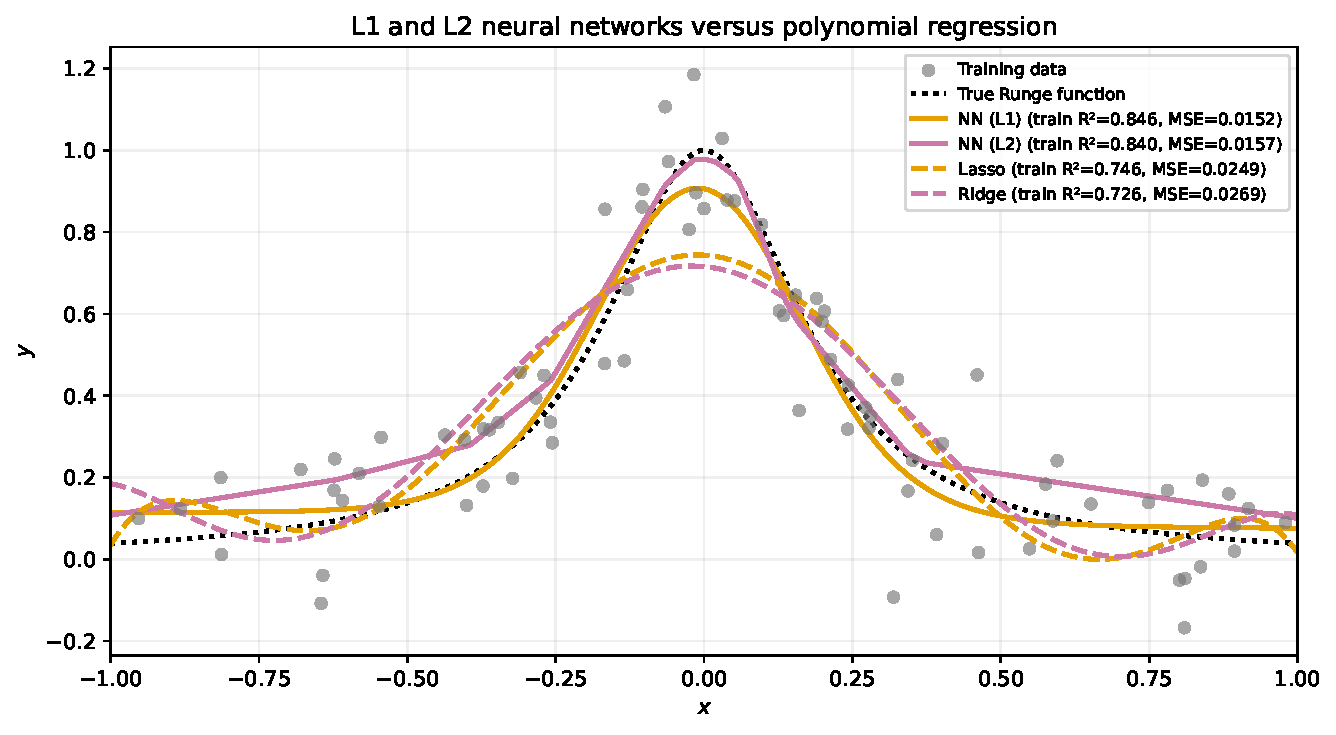
\includegraphics[width=0.85\textwidth]{part_d_runge_comparison.pdf}
    \caption{The selected regularized neural networks reproduce the Runge peak more closely than the degree-six Ridge and Lasso fits. The $\ell_1$ sigmoid network has training MSE $0.0152$ and $R^2=0.846$; the $\ell_2$ ReLU network has MSE $0.0157$ and $R^2=0.840$. The polynomial training MSE values are $0.0249$ for Lasso and $0.0269$ for Ridge. All curves are fitted to the same 80 training observations. These training scores do not establish a test-performance ranking.}
    \label{fig:regularized_runge}
\end{figure*}

We refit the selected models on all 80 training points. In Figure~\ref{fig:regularized_runge}, the networks follow the central peak more closely than the degree-six Ridge and Lasso fits. Their training MSE values are approximately $0.0152$ and $0.0157$, compared with $0.0249$ for Lasso and $0.0269$ for Ridge. The sigmoid curve is smooth, while ReLU gives a more piecewise-linear fit.


\subsubsection{Final comparison}\label{sec:regression_final_comparison}

For the final comparison, we use the CV-selected networks with no regularization, $\ell_1$ regularization and $\ell_2$ regularization. The unregularized network uses sigmoid activation, one hidden layer of 50 neurons and $\gamma=0.01$. The $\ell_1$ network also uses sigmoid and 50 neurons, with $\gamma=0.05$ and $\lambda=10^{-4}$. The $\ell_2$ network uses ReLU and 50 neurons, with $\gamma=0.01$ and $\lambda=10^{-4}$. All three networks have 151 parameters. The unregularized network has the lowest CV MSE among the three, and would be our preferred pick based on cross-validation, but we also consider the regularized networks for comparison.

After fixing these choices, we refit each network on all 80 training points and evaluate it on the 20 test points. We compare them with OLS, Ridge and Lasso using the settings selected in Project~1.

\begin{table}[t]
    \centering
    \caption{Final regression comparison. All models are fitted on 80 training observations and evaluated on the same 20 held-out test observations after selection. Polynomial CV scores are reused from Project 1. MSE excludes regularization penalties.}
    \label{tab:part_d_final_comparison}
    \begin{tabular}{lrrrrr}
        \hline\hline
        Model     & Parameters & CV MSE  & CV SE    & Test MSE & Test R2 \\
        \hline
        NN (L1)   & 151        & 0.01729 & 0.003953 & 0.01335  & 0.8924  \\
        NN (L2)   & 151        & 0.01825 & 0.002843 & 0.01661  & 0.8662  \\
        NN (none) & 151        & 0.01707 & 0.003194 & 0.01187  & 0.9043  \\
        OLS       & 11         & 0.02351 & 0.00485  & 0.03702  & 0.7017  \\
        Ridge     & 7          & 0.02895 & 0.004678 & 0.03153  & 0.7459  \\
        Lasso     & 7          & 0.02704 & 0.004996 & 0.02305  & 0.8143  \\
        \hline\hline
    \end{tabular}
\end{table}


The unregularized network gives the lowest test MSE, $0.01187$, and the highest $R^2$, $0.9043$ (Table~\ref{tab:part_d_final_comparison}). The $\ell_1$ network gives test MSE $0.01335$ and $R^2=0.8924$, while the $\ell_2$ network gives $0.01661$ and $0.8662$. All three networks outperform the polynomial models on this split. Lasso is the best polynomial model, with test MSE $0.02305$. The unregularized network's test MSE is approximately 50\% lower.

The unregularized network also has the lowest mean CV MSE, although the differences between the networks are small compared with their SE. Regularization therefore gives no improvement among these selected configurations. This does not reflect the effect of the penalties, since the activation and learning rate also differ between configurations. The test set contains only 20 points, and we do not repeat the experiment with different initializations, so the ranking may change for another split or seed.

\subsection{Classification}\label{sec:results_classification}

\begin{figure}[!htbp]
    \centering
    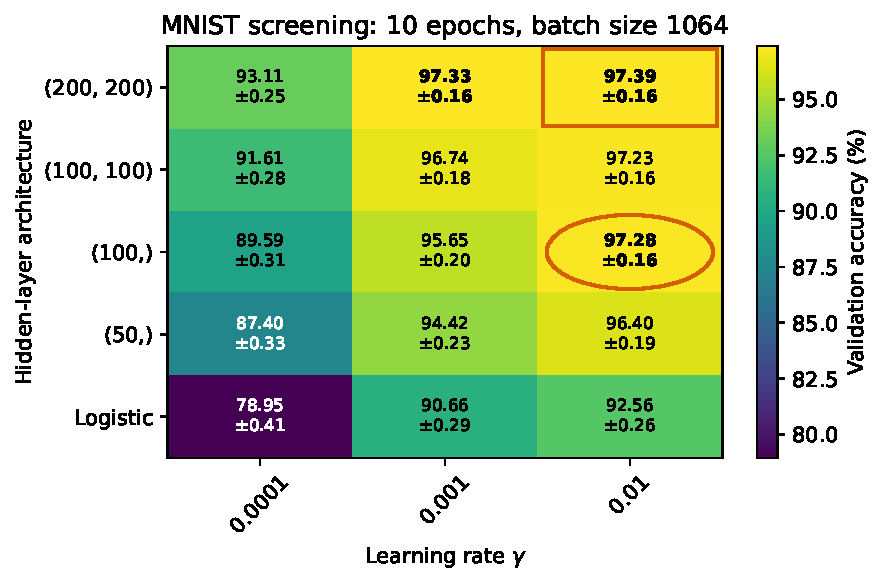
\includegraphics[width=\columnwidth]{part_e_screening.pdf}
    \caption{Hidden layers substantially improve short-run validation accuracy over the logistic baseline. At $\gamma=0.01$, one ReLU layer of 100 neurons reaches $97.28\%$, within one SE of the $97.39\%$ maximum from two layers of 200 neurons. The screening uses Adam, ten epochs, batches of 1064, 50\,000 fitting images and 10\,000 validation images. Cells show accuracy $\pm$ approximate binomial SE in percentage points. The square marks the maximum, the circle the preliminary one-SE choice, and bold cells satisfy the screening threshold.}
    \label{fig:mnist_screening}
\end{figure}

For MNIST, we first use 50\,000 images for training and 10\,000 for validation, keeping the official 10\,000 test images untouched, until the final comparison. Figure~\ref{fig:mnist_screening} shows 15 configurations trained for ten epochs with Adam, batch size 1064 and ReLU as activation function. The largest tested learning rate, $\gamma=0.01$, gives the highest accuracy for each architecture. Logistic regression reaches $92.56\pm0.26\%$, compared with $97.28\pm0.16\%$ for one ReLU layer of 100 neurons and $97.39\pm0.16\%$ for two ReLU layers of 200 neurons.

The difference between the two leading networks is about 0.11 percentage points. The smaller network is within one SE of the highest accuracy and uses 79\,510 parameters rather than 199\,210. We therefore select it at this first stage, but keep both networks for further testing. Ten epochs also favour networks that learn quickly, so we train the final candidates for longer before making the final choice.

\subsubsection{Activation functions and regularization}

\begin{figure}[!htbp]
    \centering
    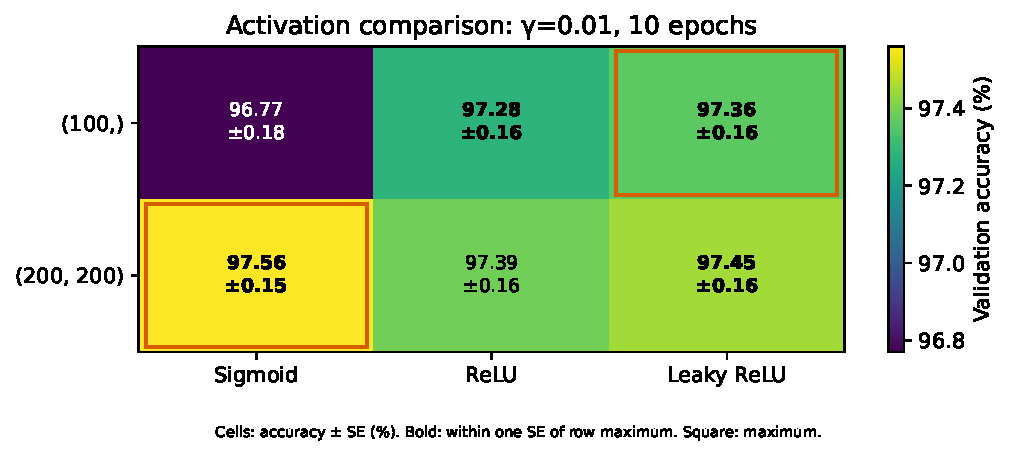
\includegraphics[width=\columnwidth]{part_e_activation_followup.pdf}
    \caption{The preferred activation depends on architecture. Leaky ReLU gives the highest validation accuracy for one hidden layer of 100 neurons, while sigmoid gives the highest for two layers of 200 neurons. All models use Adam, $\gamma=0.01$, ten epochs, batch size 1064 and no regularization. Cells show validation accuracy $\pm$ approximate binomial SE in percentage points. Squares mark row maxima; bold cells are within one SE of their row maximum.}
    \label{fig:mnist_activations}
\end{figure}

We next compare activation functions for these two architectures using the results shown in Figure~\ref{fig:mnist_activations}. With one layer of 100 neurons, Leaky ReLU reaches $97.36\%$, while sigmoid gives $96.77\%$. With two layers of 200 neurons, sigmoid instead gives the highest accuracy, $97.56\%$. The best activation therefore depends on the architecture.

\begin{figure}[!htbp]
    \centering
    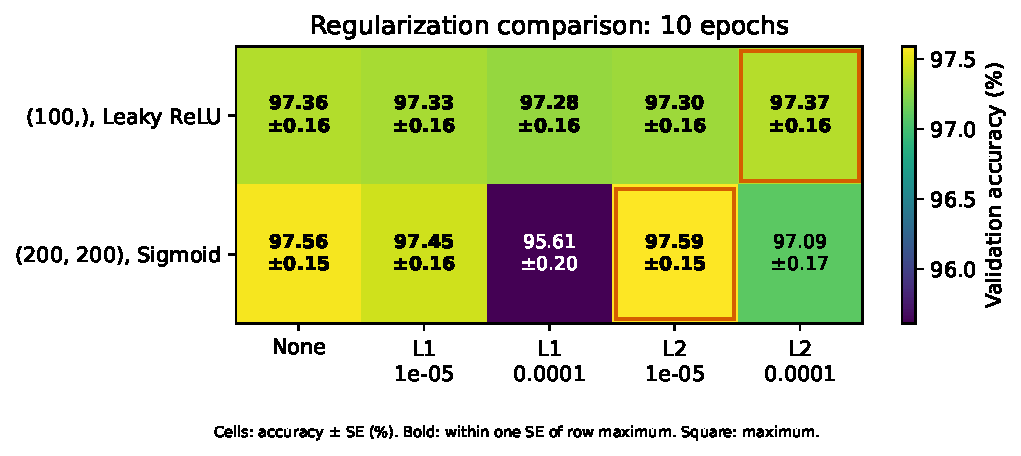
\includegraphics[width=\columnwidth]{part_e_regularization_followup.pdf}
    \caption{Weak $\ell_2$ ($\lambda=10^{-5}$) regularization gives only a small improvement over the unregularized models, while $\ell_1$ with $\lambda=10^{-4}$ reduces accuracy for the larger sigmoid network. Each architecture retains its selected activation: Leaky ReLU for one layer of 100 neurons and sigmoid for two layers of 200 neurons. All runs use Adam, $\gamma=0.01$, ten epochs and batch size 1064. Cells show validation accuracy $\pm$ approximate binomial SE in percentage points. Squares mark row maxima; bold cells are within one SE of their row maximum.}
    \label{fig:mnist_regularization}
\end{figure}


Regularization gives only small improvements in these ten-epoch runs. For the larger sigmoid network, accuracy increases from $97.56\%$ without a penalty, to $97.59\%$ with $\ell_2$ and $\lambda=10^{-5}$. This difference is smaller than its SE of approximately 0.15 percentage points. Increasing the $\ell_1$ strength to $10^{-4}$ reduces accuracy to $95.61\%$. Stronger regularization can therefore also reduce performance.

After the activation tests, regularization tests and longer training, the one-SE rule selects the larger sigmoid network with two hidden layers of 200 neurons, $\gamma=0.01$ and $\ell_2$ strength $10^{-5}$. We select epoch 27, with validation accuracy $98.18\%$. Logistic regression is selected at epoch 6 with $92.59\%$, a difference of 5.59 percentage points.

\subsubsection{Training and validation accuracy}
\begin{figure}[!htbp]
    \centering
    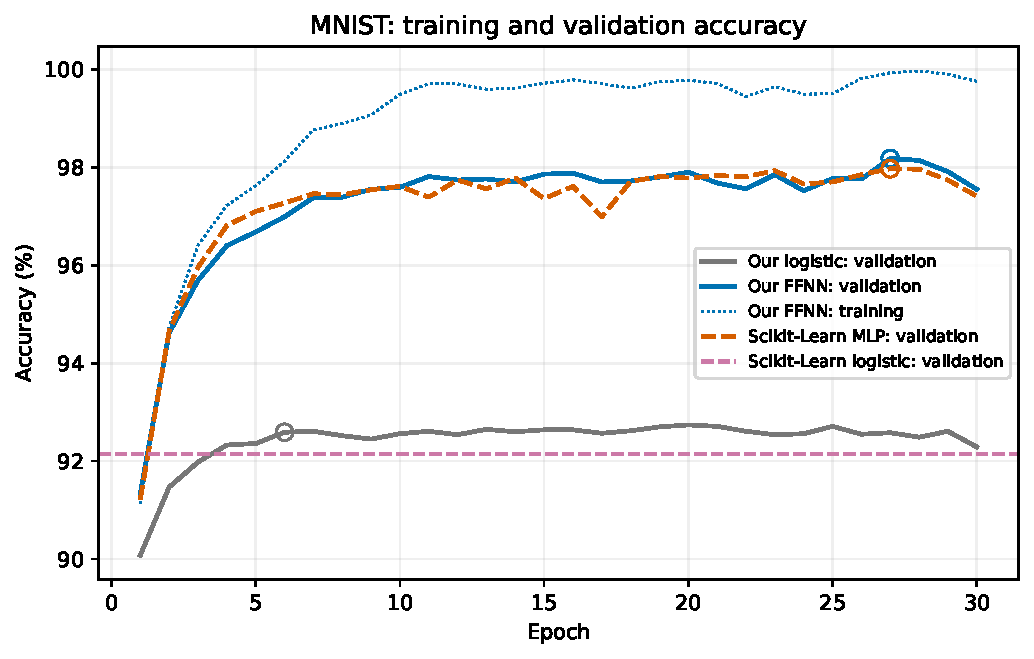
\includegraphics[width=0.5\textwidth]{part_e_learning_curves.pdf}
    \caption{The hidden-layer networks reach similar validation accuracy near $98\%$, compared with approximately $92$--$93\%$ for logistic regression. Our FFNN's training accuracy approaches $100\%$, leaving a gap to validation accuracy. Curves use 50\,000 training images and 10\,000 validation images. Both hidden-layer networks have two sigmoid layers of 200 neurons, Adam with $\gamma=0.01$, $\ell_2$ strength $10^{-5}$ and batch size 1064. Circles mark the selected epoch counts. Scikit-learn models are dashed; we dont have the accuracy across epochs for Sklearn's logistic regression.}
    \label{fig:mnist_learning_curves}
\end{figure}

Figure~\ref{fig:mnist_learning_curves} compares the training histories before the final refit. Our FFNN and Scikit-learn's MLP follow similar validation curves and reach approximately $98\%$, while both logistic models remain near $92$-$93\%$. The hidden layers therefore give a clear improvement over logistic regression. Our FFNN's training accuracy approaches $100\%$, while validation accuracy stays near $98\%$. Learning the training images more closely therefore does not give the same improvement on unseen validation images.

We select epoch 27 for our FFNN and the library MLP, and epoch 6 for our logistic model. The MLP uses the same two hidden layers of 200 neurons, sigmoid activation, learning rate and $\ell_2$ setting as our selected FFNN. Its sigmoid activation is used in the hidden layers; the output uses softmax for multiclass classification. Scikit-learn's logistic model is shown as a horizontal reference because it does not provide the epoch history.

\subsubsection{Final comparison}

\begin{table*}[t]
    \centering
    \caption{MNIST test results after refitting fixed models on all 60,000 training images. Accuracy and macro-F1 are fractions. Times are refit wall times. Selected FFNN: Sigmoid, gamma=0.01, L1=0, L2=1e-05, 27 epochs. MLP: Sigmoid, gamma=0.01, L2=1e-05, 27 epochs.}
    \label{tab:part_e_final_comparison}
\begin{tabular}{llrrrr}
\hline\hline
Model & Architecture & Params & Time (s) & Test acc. & Macro F1 \\
\hline
Our logistic & () & 7850 & 8.045 & 0.9245 & 0.9235 \\
Our FFNN & (200, 200) & 199210 & 89.7 & 0.9788 & 0.9787 \\
Scikit-Learn logistic & () & 7850 & 540 & 0.9252 & 0.9242 \\
Scikit-Learn MLP & (200, 200) & 199210 & 43.87 & 0.9766 & 0.9766 \\
\hline\hline
\end{tabular}
\end{table*}


After fixing the configurations and epoch counts, we refit all four models on the full 60\,000 training images, including the former validation images. We then evaluate them on the same 10\,000 test images (Table~\ref{tab:part_e_final_comparison}). Our FFNN gives test accuracy $97.88\%$ and macro-$F_1=0.9787$, compared with $92.45\%$ and $0.9235$ for our logistic model. Adding hidden layers improves test accuracy by 5.43 percentage points.

The Scikit-learn models give similar results. Its logistic model reaches $92.52\%$ test accuracy, only 0.07 percentage points above ours. Its MLP reaches $97.66\%$ and macro-$F_1=0.9766$, compared with $97.88\%$ for our FFNN. This difference corresponds to 22 additional correct predictions out of 10\,000.

Our FFNN takes approximately 90 seconds to refit, compared with 44 seconds for the library MLP. Our logistic model takes approximately 8 seconds, while Scikit-learn's takes 540 seconds (not representative). These are the wall times for the specific solvers and stopping settings used here. In particular, our logistic model uses six epochs, while the library model uses a different solver and stopping settings, so the times do not represent equal training budgets.

\subsubsection{Classification errors}

The confusion matrix in Figure~\ref{fig:mnist_confusion} shows 9788 correct predictions and 212 errors. The most frequent error is $7\!\to\!2$, with 17 images, followed by $7\!\to\!9$ and $5\!\to\!3$, with 12 images each. Digit 7 has 976 correct predictions out of 1028 images, giving recall approximately $94.94\%$. For comparison, digit 1 has 1130 correct predictions out of 1135, or $99.56\%$. The overall accuracy therefore hides differences between digits. The cells contain counts, so their values also depend on how many test images each digit has.

\begin{figure}[!htbp]
    \centering
    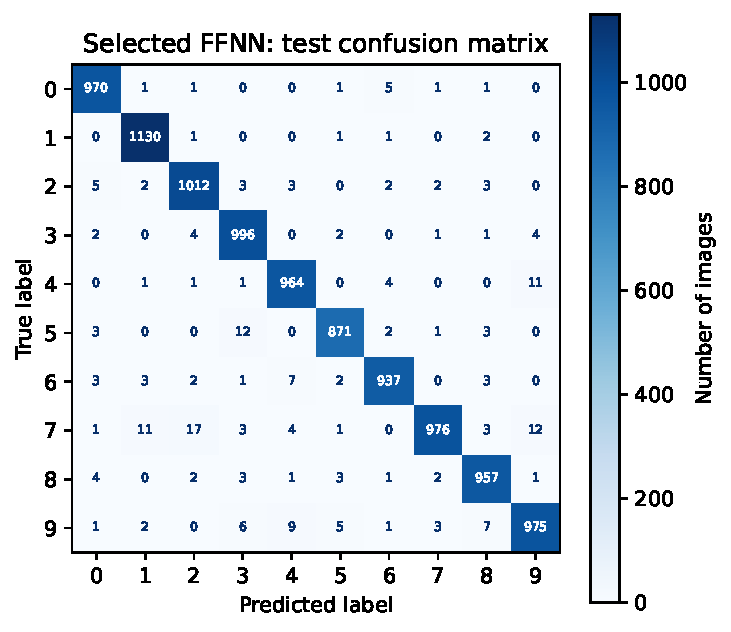
\includegraphics[width=0.5\textwidth]{part_e_confusion_matrix.pdf}
    \caption{The selected FFNN correctly classifies 9788 of the 10\,000 test images. Cells show image counts, with true digits in rows and predicted digits in columns. The largest off-diagonal count is 17 for $7\!\to\!2$, followed by 12 each for $7\!\to\!9$ and $5\!\to\!3$. There are also 11 errors from $4\!\to\!9$ and nine from $9\!\to\!4$.}
    \label{fig:mnist_confusion}
\end{figure}

\begin{figure}[!htbp]
    \centering
    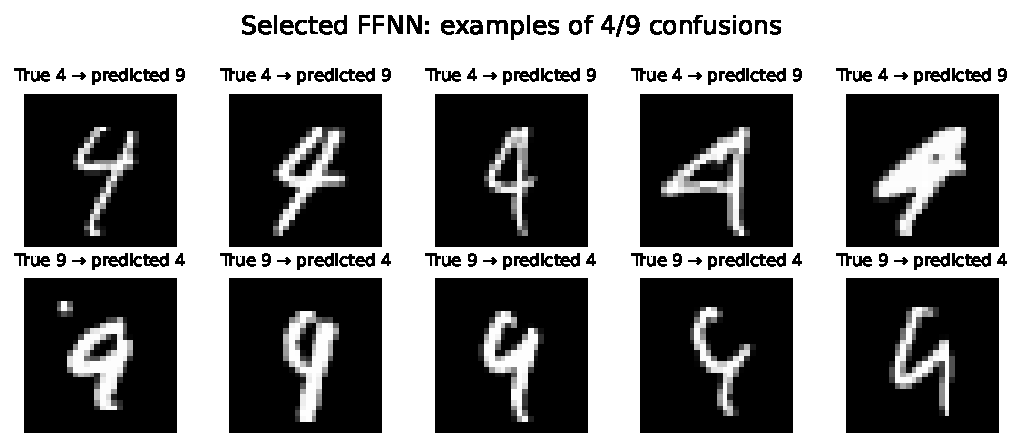
\includegraphics[width=0.5\textwidth]{part_e_confused_4_9.pdf}
    \caption{Some misclassified fours and nines have similar shapes, making them difficult to distinguish visually. The upper row shows true fours predicted as nines; the lower row shows true nines predicted as fours}
    \label{fig:mnist_four_nine}
\end{figure}

The network also confuses digits 4 and 9: 11 fours are predicted as nines, and nine nines are predicted as fours. Figure~\ref{fig:mnist_four_nine} shows five randomly selected examples of each error, using seed 2026. Looking at the handwriting, some of these mistakes are understandable. Some fours are closed at the top and look like nines, while some nines are open at the top and look like fours. A few are difficult to tell apart even by humans, but others look clearer.

\section{Conclusion}\label{section:conclusion}

We implemented a feed-forward neural network for Runge regression and MNIST classification, using backpropagation and the optimization methods from Project~1. In polynomial regression, we choose the features through powers of $x$. A neural network instead learns features from the input through its hidden layers. The universal approximation theorem (section \ref{section:methods}) shows that a sufficiently large network can approximate a continuous function, but does not guarantee that training finds the required weights or that the model generalizes well.

For Runge regression, adding layers and neurons did not consistently improve performance. The unregularized sigmoid network with one hidden layer of 50 neurons gave the lowest test MSE, $0.01187$, and $R^2=0.9043$. All three selected networks outperformed the polynomial models on this split. Regularization gave no improvement among the selected configurations. With only 20 test points, the ranking may change for another split or initialization. Polynomial regression still remains a useful, inexpensive benchmark.

Architecture and optimization must be considered together. Adam reached low training MSE over a broader range of learning rates than RMSProp. Deeper sigmoid networks often gave higher CV MSE, consistent with vanishing gradients, although we did not check with more epochs. We selected hyperparameters using cross-validation for regression and a separate validation set for MNIST. The one-SE rule favours simpler models with similar validation performance, while excessively strong regularization can cause underfitting.

For MNIST, the selected network with two sigmoid hidden layers of 200 neurons and weak $\ell_2=10^{-4}$ regularization reached test accuracy $97.88\%$ and macro-$F_1=0.9787$. Our logistic model reached $92.45\%$ accuracy, while Scikit-learn's MLP reached $97.66\%$. Hidden layers therefore improved classification over the linear baseline. The confusion matrix shows differences between digits, with $7\!\to\!2$ the most frequent error. The confused fours and nines also illustrate how similar handwriting can make some images difficult to distinguish.

Computing resources limited our search and training time. Future work could use more epochs for both tasks, with validation monitoring and early stopping to limit overfitting. Repeated runs with different seeds would help assess sensitivity to initialization. For MNIST, a convolutional neural network (CNN) could use local filters and shared weights to learn the spatial patterns in the images more directly.


\bibliography{biblio}

\onecolumngrid
\newpage

\section{Appendix}
\appendix
\section{Supplementary figures}\label{app:regression_extra}


\begin{figure}[!htbp]
    \centering
    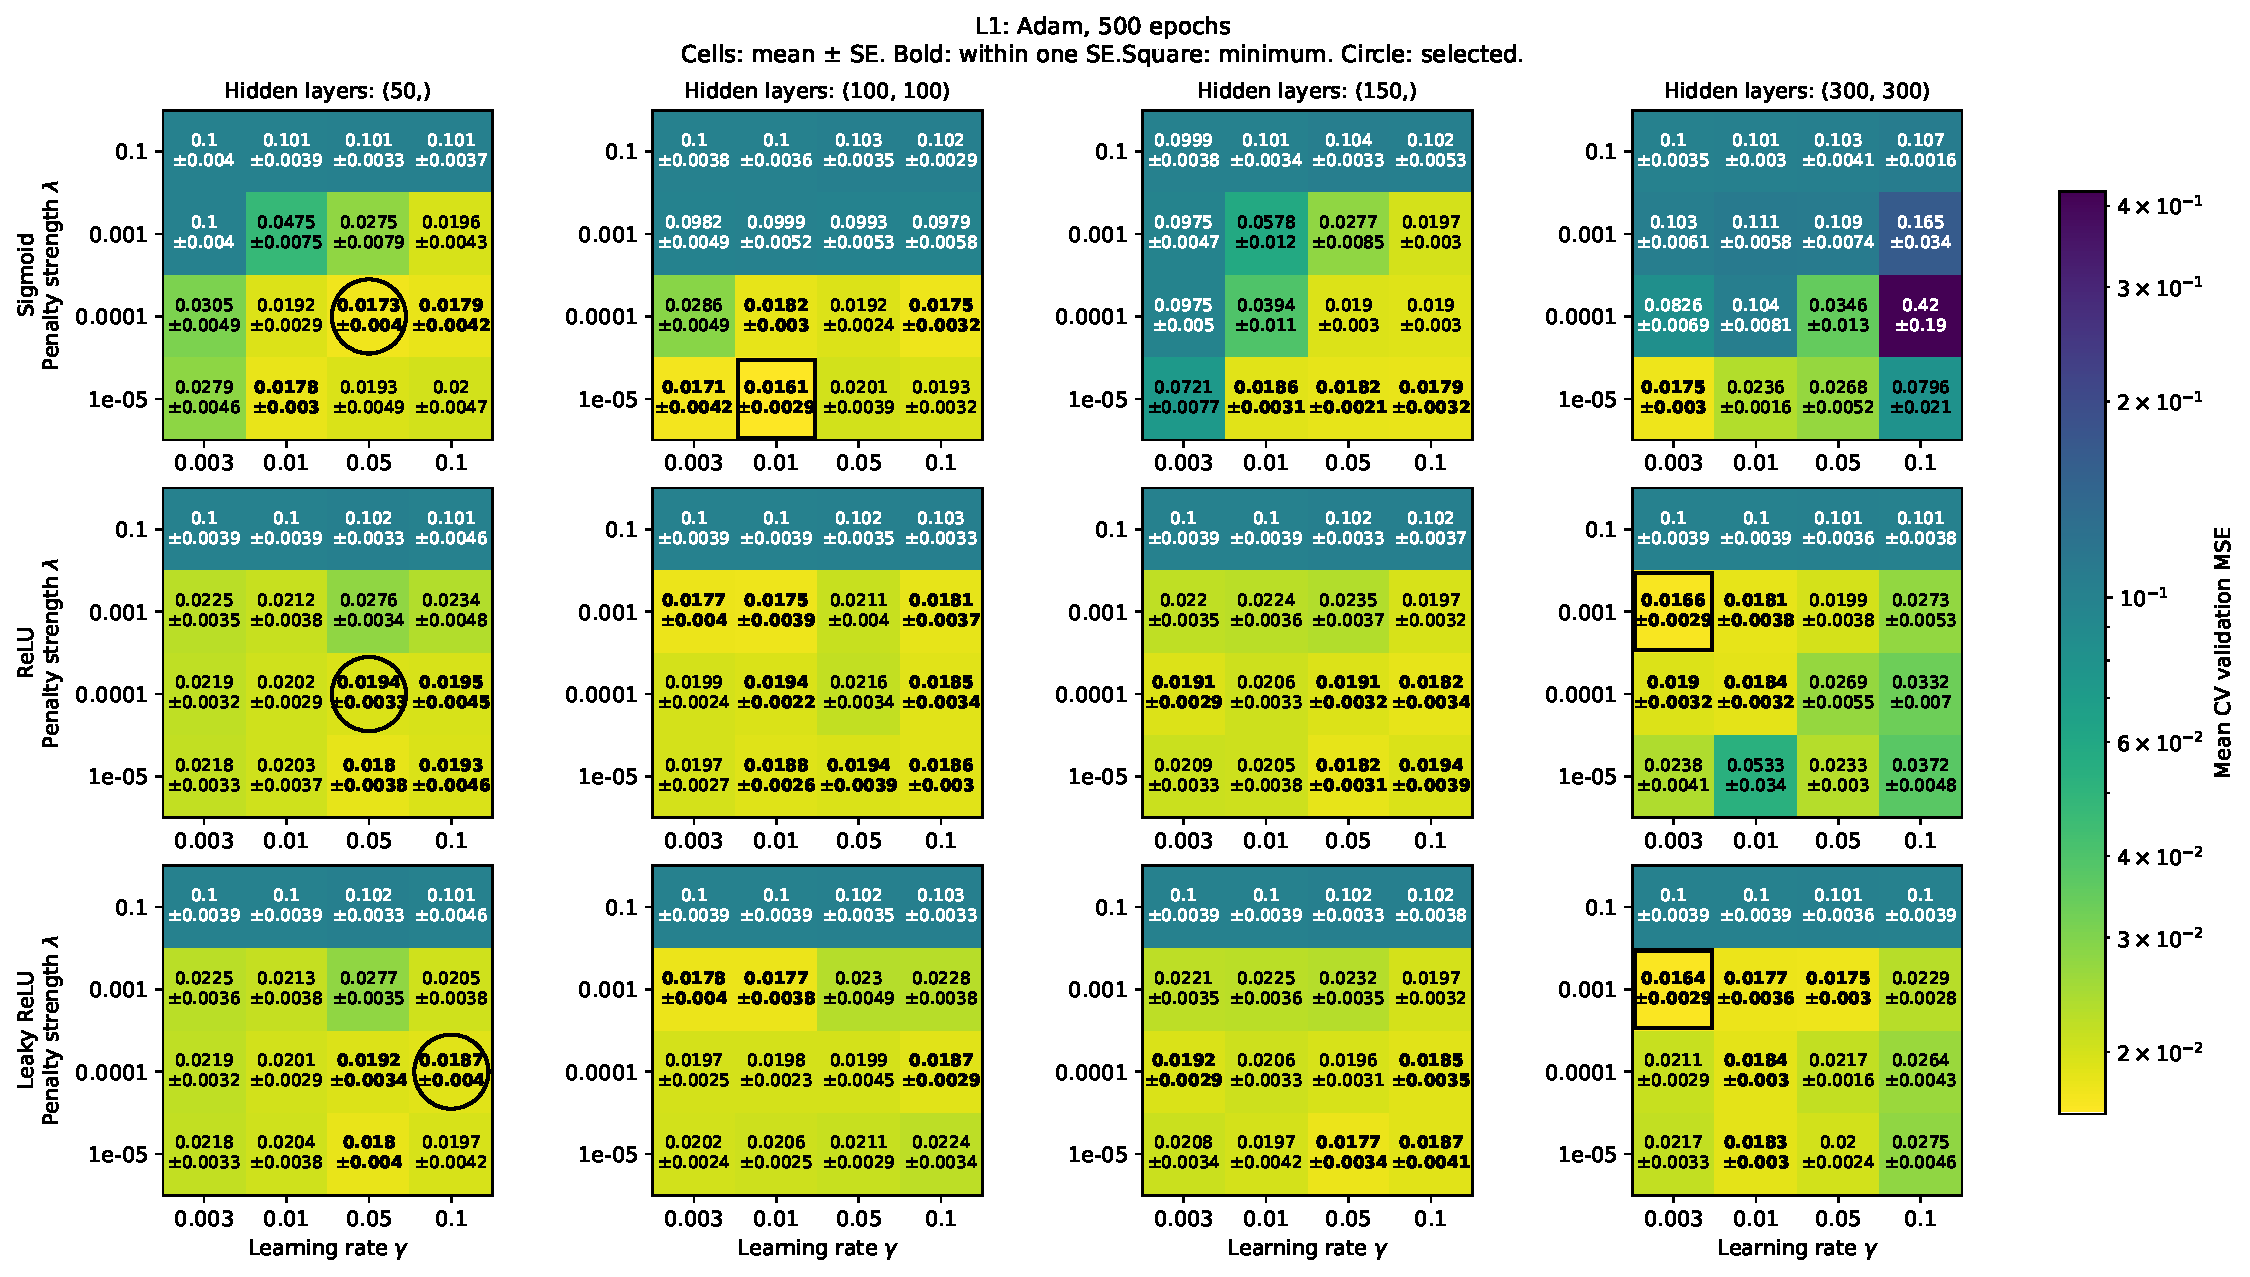
\includegraphics[width=\textwidth]{part_d_l1_cv.pdf}
    \caption{The full $\ell_1$ search shows interactions between architecture, activation, learning rate and penalty strength. Strong regularization ($\lambda=0.1$) generally produces CV MSE near $0.10$, while weaker penalties allow errors near $0.016$--$0.02$ in suitable regions. The widest sigmoid architecture is particularly sensitive to large learning rates. Each configuration uses Adam, 500 epochs, batch size 16 and five-fold training-data CV. Cells show validation MSE $\pm$ SE; bold marks eligibility under the activation-specific one-SE threshold, squares mark minima and circles mark the selected configurations.}
    \label{fig:appendix_l1_search}
\end{figure}

\begin{figure}[!htbp]
    \centering
    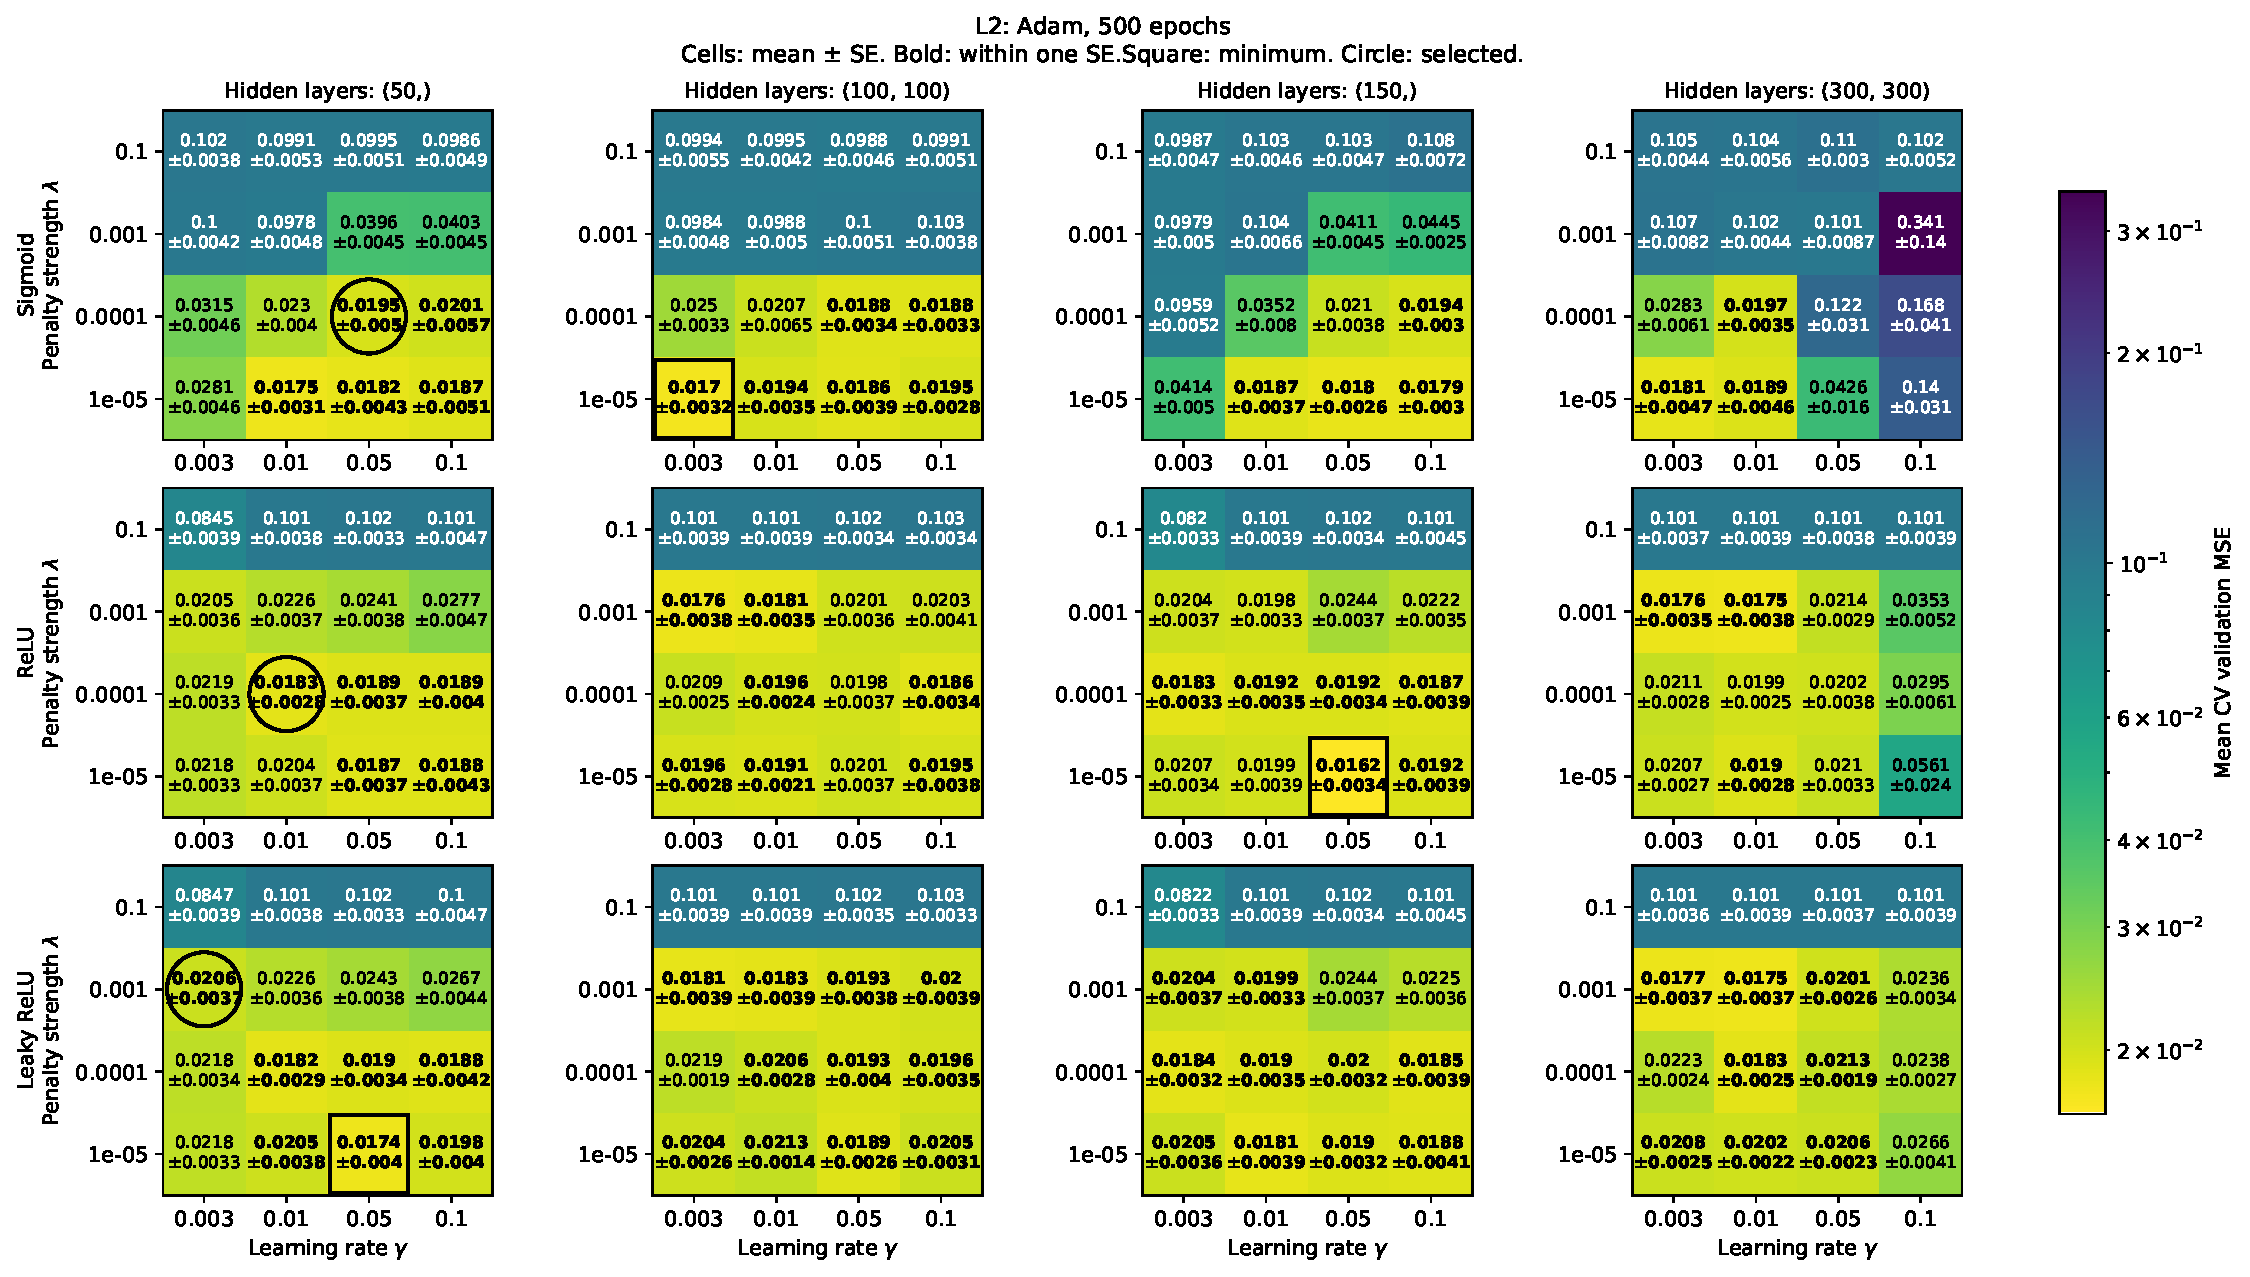
\includegraphics[width=\textwidth]{part_d_l2_cv.pdf}
    \caption{The full $\ell_2$ search also contains broad high-error regions at strong regularization and low-error regions at weaker penalties. Larger architectures do not uniformly improve validation performance, and learning-rate sensitivity remains visible. Models use Adam, 500 epochs, batch size 16 and five-fold training-data CV. Cells show validation MSE $\pm$ SE. Selection markers have the same meanings as in Figure~\ref{fig:appendix_l1_search}. Colour scales are fitted separately for the two penalty figures, so numerical cell values should be used for comparisons between them.}
    \label{fig:appendix_l2_search}
\end{figure}
\clearpage

\section{Use of AI/LLM tools}
\subsection{Tools used}
\begin{itemize}
    \item GitHub Copilot (VS Code, throughout) for code autocompletion
    \item ChatGPT (chatgpt.com, October-November 2026) for grammar corrections, rephrasing, and improving the fluency and clarity of the text. Also generated plots for the report, and used for code.
    \item DeepSeek (deepseek.ai, November 2026) used to generate TikZ figures for the report
\end{itemize}

\subsection{Text writing and editing.}
\begin{tabular}{llp{7cm}}
    Section          & Level & Notes                                           \\ \hline
    Abstract         & 1-2   & some rephrasing and language corrections        \\
    Introduction     & 2     & rephrased for clarity; ideas and structure ours \\
    Theory / Methods & 2     & rephrased for clarity; ideas and structure ours \\
    Results          & 2     & rephrased for clarity; ideas and structure ours \\
    Conclusion       & 2     & rephrased for clarity; ideas and structure ours \\
\end{tabular}

\subsection{Code generation and assistance.}

\begin{tabular}{llp{7cm}}
    Folder/file                                & Level & Description                                                                                                             \\ \hline
    \texttt{network/}                          & 1     & Copilot autocomplete only                                                                                               \\
    \texttt{optimizers/}                       & 1     & Copilot autocomplete only                                                                                               \\
    \texttt{training/}                         & 1     & Copilot autocomplete only                                                                                               \\
    \\
    \texttt{utils/}                            & 1     & Copilot autocomplete only                                                                                               \\
    \texttt{scripts/part\_b.py-part\_e.py}     & 2-4   & ChatGPT assisted with code generation and logic for parts C to E. Adjusted the code skeleton to fit our implementation. \\                                                                        \\
    \texttt{tests/}                            & 3-4   & ChatGPT generated the tests. Minor modifications were made to fit our implementation.                                   \\                                                                                                                                                                                               \\
    \texttt{notebooks/Project2\_results.ipynb} & 2-4   & ChatGPT helped with plotting of the heatmaps, and all plots for part E.                                                 \\
\end{tabular}

\end{document}
